\documentclass[12pt]{ociamthesis}  % default square logo 
%\documentclass[12pt,beltcrest]{ociamthesis} % use old belt crest logo
%\documentclass[12pt,shieldcrest]{ociamthesis} % use older shield crest logo

%load any additional packages
\usepackage{amssymb}
\usepackage{setspace}
\usepackage{amsmath}
\onehalfspacing
\usepackage[a4paper, margin=2.5cm]{geometry}
\usepackage{fontspec}
\setmainfont{Times New Roman}
\usepackage{graphicx}
\usepackage[backend=biber, style=apa]{biblatex}
\addbibresource{refs.bib}
\addbibresource{software.bib}
\graphicspath{ {./images/} }
\usepackage{titlesec}
\usepackage{lipsum}
\usepackage{sectsty}

\titleformat{\chapter}[display]
  {\normalfont\bfseries}{}{0pt}{\Large}

\chapterfont{\fontsize{12}{15}\selectfont}
\sectionfont{\fontsize{12}{15}\selectfont}
\subsectionfont{\fontsize{12}{15}\selectfont}
\subsubsectionfont{\fontsize{12}{15}\selectfont}

%input macros (i.e. write your own macros file called mymacros.tex 
%and uncomment the next line)
%\include{mymacros}

\title{Changes in brain hierarchy following acute and chronic use of DMT and cannabis}   %note \\[1ex] is a line break in the title

\author{Robert Tromm | i6272405}             %your name
%\college{}  %your college

%\renewcommand{\submittedtext}{change the default text here if needed}
\degree{MSc Cognitive and Clinical Neuroscience, Specialization in Drug Development \& Neurohealth}     %the degree
\degreedate{November 2023}         %the degree date

%end the preamble and start the document
\begin{document}

%this baselineskip gives sufficient line spacing for an examiner to easily
%markup the thesis with comments
%\baselineskip=18pt plus1pt

%set the number of sectioning levels that get number and appear in the contents
\setcounter{secnumdepth}{3}
\setcounter{tocdepth}{3}


\maketitle                 % create a title page from the preamble info
\begin{dedication}
    To my family for paving a path of abundance for their children.\\
    To my chosen family for their passion, support, and loyalty.
\end{dedication}        % include a dedication.tex file
\begin{acknowledgements}

I would be remiss not to begin by expressing my deep gratitude to Oxford for the vast natural beauty and awe-inspiring architecture it has blessed me with in the last few months. My time here has changed me in ways I have not yet begun to process, akin to the grandeur of altered experiences embedded in the pages of this thesis. To Jan, for the trust you placed in me. Overwhelmed, I stepped into your office;  with just a few words you introduced me to scientific passions I had no idea were within me. To Morten, for welcoming me with open arms into the Eudaimonia community, and for teaching me scientific rigor, curiosity, criticality, and wisdom. To my family, for the excitement they have for my journey through this academic life. Our lives are so different, and yet you have always shown me unconditional support and understanding.

To the wider Eudaimonia community for their generous and gracious support, advice, and friendship. Thank you to Leonardo for solving every silly roadblock I ran into in the darkness of the back office. To Kat, Elvira, Gustavo, Dimitri, Pedro, Fernando, Shamil, Robin, and Joana for the kindness, questions, and critique which allowed me to repair the cracks in my work, and my thinking about the brain and mind.

Thank you to the friends I have made since my time in Oxford, whose limitless optimism, curiosity, and love have changed the way I think about friendship, science, and life, and kept me grounded as my mind tripped and fell over the complexities of entropy and hierarchy. Thank you to Michael, Kenneth, Fil, Clayton, Will, Elin, Sebastian, Victoria, and Marilena, whose presence has given me more than can be expressed in words, or at least the limited space I have here.

Last but not least, to Maastricht and the psychopharmacology team. To Pablo for holding my hand with patience as I took my first steps in the blinding, expansive world of neuroimaging. A summer I very well could have spent traveling was spent behind my laptop, bashing keys with frustration as FSL threw errors for the thousandth time. I would not change that for anything. Thank you to Petr, who saw the light in me and challenged me to let it out. And to Baptiste, Mila, and Aedan for every moment shared, whether a long night in the library or in Cafe Zondag.
\end{acknowledgements}  % include an acknowledgements.tex file
\begin{abstract}
    Abstract goes here.
\end{abstract}          % include the abstract

\begin{romanpages}          % start roman page numbering
\tableofcontents            % generate and include a table of contents
\listoffigures              % generate and include a list of figures
\end{romanpages}            % end roman page numbering

%now include the files of latex for each of the chapters etc

\chapter{Introduction}
    Psychedelics, including drugs such as psilocybin (4-PO-DMT), lysergic
acid diethylamide (LSD), and dimethyltryptamine (DMT), an ingredient in
the ritual brew ayahuasca, have seen a massive resurgence in medical and
scientific interest in the last decade. These compounds induce
significant altered states of consciousness, characterized by vivid
imagery, the sense of being in another reality, and dissolution or
loosening of the ego, or one's sense of self. Previous research has
shown psychedelics to have lasting impacts on personality and mental
health outcomes \parencite{Barbosa2009,Griffiths2008}.
Personality traits are considered to be rigid and inflexible in healthy
adults, and despite this psychedelics have been shown to increase trait
openness several months after an acute experience \parencite{Griffiths2011,MacLean2011, McCrae1997}. Evidence is
mounting that psychedelics can improve outcomes for a variety of
conditions, including depression \parencite{Raison2023}, OCD \parencite{Moreno2006}, smoking addiction \parencite{Johnson2017}, and alcohol
use disorder \parencite{Bogenschutz2015}. The strongest evidence for the
therapeutic use of psychedelics lies with depressive and anxiety
symptoms associated with life-threatening illnesses, such as cancer \parencite{Griffiths2008,Griffiths2006,Grob2011}.
These results highlight the need for further research into their effects
on the brain.

The propensity of psychedelics to induce significant altered states also
makes them an interesting candidate to assist in understanding normal
and abnormal brain function and identifying the neural correlates of
consciousness. Previous work has showed that psychedelics modulate
emotion \parencite{Roseman2019}, sense of self \parencite{Lebedev2015}, perceptual processing \parencite{Kometer2016}, and
increase feelings of connectedness \parencite{Carhart-Harris2018b}. A large body
of evidence indicates that psychedelics trigger these effects via 5-HT2a
agonism \parencite{Nichols2016}, which are localized in the cortex, primarily in
the association cortices \parencite{Nichols2016,Weber2010}. It is not
well-known what the downstream effects of 5-HT2a agonism are with regard
to global brain function, though the rate of research has been growing
steadily. Recent work has shown that the therapeutic effects of
psychedelics, in rodents, are mediated by TrkB agonism \parencite{Moliner2023}. A convergent body of research has indicated that psychedelics
increase measures of brain complexity during the acute psychedelic
experience \parencite{Lebedev2016,Tagliazucchi2014,Viol2017}. These results build support for the theory that, during
normal waking consciousness, the human brain operates at
sub-criticality, or perfect criticality \parencite{Carhart-Harris2014}.
Criticality has been shown to play a role in a variety of processes in
nature, and in the brain it has been speculated to play a role in
neuronal avalanches \parencite{Beggs2003}. Early studies indicate that
psychedelics suppress the default mode network (DMN), decreasing
within-network integrity and segregation from other resting-state
networks \parencite{Buckner2008,Carhart-Harris2012,Johnson2019,Muller2018,Petri2014,Roseman2014,Tagliazucchi2014,Timmermann2023}. Furthermore,
decoupling between the DMN and medial temporal lobes has been shown
\parencite{Carhart-Harris2014}, which has led to the suggestion that the
effects of psychedelics are mediated by suppression and desegregation of
networks in the association cortex \parencite{Girn2022}.

The evaluation of long-term outcomes of psychedelic use, as well as the
development of an understanding of how psychedelics modulate brain
dynamics long-term, has not been extensively demonstrated. \textcite{Bouso2015} found significant differences in cortical thickness in midline
structures of the brain, with thinning in the middle frontal gyrus,
inferior frontal gyrus, precuneus, superior frontal gyrus, superior
occipital gyrus, and posterior cingulate cortex (PCC), a key node of the
default mode network (DMN). Thickening was found in
the precentral gyrus and anterior cingulate cortex. Importantly, the
medial prefrontal cortex (mPFC), ACC, and PCC have been associated with
the acute effects of psychedelics \parencite{Riba2006}, and disruption of
the default mode network is a key, convergent finding in psychedelic
neuroimaging studies \parencite{Carhart-Harris2017a,McCulloch2022}. Furthermore, previous work has demonstrated a significant
increase in resting-state functional connections across the brain one
month after psilocybin use \parencite{Barrett2020}.

It's believed that psychedelics shift brain dynamics into a more
flexible, diverse, and sensitive mode that is more tuned for information
sharing and propagation \parencite{Atasoy2017,Carhart-Harris2014, Carhart-Harris2017, Daws2022, Girn2022, Girn2023, Lord2019, Singleton2022, Tagliazucchi2014, Tagliazucchi2016, Timmermann2023} The state of unconstrained cognition induced by psychedelics has been previously conceptualized as a
flattening of the attractor landscape -- the brain
has a reduced tendency to exhibit metastability within potentially
maladaptive local minima states, and is thus able to more easily move
between metastable local minima \parencite{Carhart-Harris2007, Carhart-Harris2014, Kraehenmann2017, Kraehenmann2017a, Girn2023, Daws2022, Singleton2022}. This is consistent with the REBUS (`RElaxed Beliefs Under
Psychedelics') model of psychedelic action as proposed by \textcite{Carhart-Harris2019a}, which proposes that psychedelics increase
entropy in the brain, resulting in `critical primary states' which allow
for the relaxation of priors and decreased rigidity of thinking and
cognition. Entropy is an information-theoretic measure derived from
thermodynamics which indexes the fundamental temporal complexity or
diversity of a trajectory of the dynamics of a system and the
unpredictability of the trajectory, specifically the
relative frequency of values that a signal in a system takes on \parencite{Girn2023}. It is
often characterized more simply as disorder or randomness in a system.
Similarly, it is thought that psychedelics flatten the global functional
hierarchy of the brain by increasing crosstalk between hierarchical
extremes \parencite{Girn2022, Timmermann2023}. Hierarchy here is
defined as the directional asymmetry of information flow throughout the
brain, or alternatively, the rigidity and stratification of the network \parencite{Kringelbach2023}. However, it is difficult to analyze
these theories directly, and thus far research has failed to
differentiate the action of psychedelics with respect to specific
region- or network-wise changes \parencite{Girn2023}.

Network theory offers a plethora of approaches to the study of the brain
as a complex system, and allows for direct examination of the
hierarchical organization of the brain under psychedelics. Previous
research has pointed toward the idea that the brain, rather than acting
on the world purely through interpretation of environmental stimuli, is
constrained by its own dynamics \parencite{Buzsaki2019}. Irreversibility is then
a measure of how the external environment drives internal brain dynamics \parencite{Buzsaki2019, Deco2022, Kringelbach2023}. By
measuring the irreversibility of brain processes, we can estimate the
extent to which the environment drives intrinsic dynamics, from there
deriving insights about the hierarchical organization of the brain.
Previously, \textcite{Kringelbach2023} showed improved sensitivity of
irreversibility over time-averaged functional connectivity in
differentiating between rest and movie-watching conditions with
effective connectivity derived from irreversibility over functional
connectivity alone, indicating that asymmetry in information flow better
captures features of brain dynamics related to distinct states of
consciousness. A dynamics-based mechanistic
explanation of psychedelic action is especially relevant because of the
preliminary evidence indicating that changes in dynamics predict
psychological and therapeutic outcomes. For example, the degree to which
a participant has a mystical experience in a psychedelic session
predicts both changes in openness to experience 
and increases in entropy \parencite{MacLean2011, Lebedev2016}.

Here we combine the estimation of entropy production in the brain,
irreversibility, with graph theory to examine changes in the functional
hierarchical organization of the brain after ayahuasca in a naturalistic
study with 24 healthy members of Santo Daime, and DMT in a
placebo-controlled study with 17 healthy volunteers with previous
psychedelic experience. In contrast to previous work, users of ayahuasca
in the original study are extreme with regard to lifetime use of
psychedelics (mean = 564, SD = 650). Our main objective was to establish
whether psychedelics had an effect on the functional hierarchical
organization of the brain, and furthermore whether chronic use of
psychedelics alters propensity for changes in hierarchical organization
and baseline structure. In line with the REBUS and entropic brain models
of psychedelic action, we hypothesized that both psychedelics would
result in a flattening of the hierarchy under psychedelics \parencite{Carhart-Harris2014,Carhart-Harris2019}.
Furthermore, we contrast these changes with changes in hierarchical
organization in chronic and occasional users of cannabis. Previous work
in psychedelic research has been limited by the lack of contrast
analyses -- while novel findings are plentiful and leverage a variety of
techniques which converge on similar results, discriminant validity is
lacking. We sought to examine how psychedelics might alter the
hierarchical organization of the brain differently than cannabis in both
chronic and occasional users, especially given the participants under
ayahuasca had considerably more lifetime experience than DMT users.

    \chapter{Methods}
\section{Data acquisition and preprocessing}
\subsection{Occasional and chronic users of cannabis} 

\textbf{Ethics statement}:
This study was conducted according to the code of ethics on human
experimentation established by the declaration of Helsinki (1964) and
amended in Fortaleza (Brazil, October 2013). The study was approved by
the Academic Hospital and University's Medical Ethics Committee (Medical
ethical review board Academic Hospital Maastricht/ Maastricht
University). All participants gave written informed consent. The Dutch
Drug Enforcement Administration gave a permit for the acquisition,
storage, and administration of cannabis.

\textbf{Participants}: The data acquisition protocols were described in
detail in a previous paper \parencite{Ramaekers2022}. 43 healthy
participants with previous experience using cannabis were scanned. For
the occasional group, occasional usage was characterized as between one
time a month and three times a week. For the chronic group, chronic
usage was characterized as at least four times a week. Both were
considered only if usage was for the past year. The study was conducted
according to a double-blind, placebo-controlled, mixed cross-over design
in cannabis users (N=43). Each participant received cannabis placebo and
cannabis (300 ug/kg THC) on separate days, separated by a minimum
wash-out period of 7 days. Treatment orders were randomly assigned to
participants.

Participants received two resting state scans at 15 minutes and 36
minutes after inhalation. The current study was registered in the
Netherlands trial register (NTR4894, first date of registration
7/11/2014). Participants in the occasional group were instructed to
refrain from drug use, including cannabis (\textgreater7 days) and
alcohol (\textgreater14 hours) prior to the testing day. Participants in
the chronic group were given the same instructions, but instructed to
refrain from cannabis use only up until 24h before testing day.

\textbf{Neuroimaging acquisition for fMRI}: Participants underwent a
resting state functional MRI. Images were acquired on a MAGNETOM 7T MR
scanner. A total of 258 whole-brain EPI volumes were acquired at rest
(TR = 1400ms; TE = 21ms; flip angle = 60 degrees; oblique acquisition
orientation; interleaved slice acquisition; 72 slices; slice thickness =
1.5mm; voxel size = 1.5 x 1.5 x 1.5 mm). During scanning, participants
were shown a black cross on a white background and were instructed to
focus on the cross while attempting to clear the mind.

Results related to the cannabis data included in this manuscript come
from analyses performed using CONN (RRID:SCR\_009550) release 22.a and
SPM (RRID:SCR\_007037) release 12.7771 \parencite{Nieto-Castanon2022,Penny2007,Whitfield-Gabrieli2012}.

\textbf{Preprocessing:} Preprocessing was performed in line with \textcite{Luppi2021}. Functional and anatomical data were
preprocessed using a flexible preprocessing pipeline including
realignment with correction of susceptibility distortion interactions,
slice timing correction, outlier detection, direct segmentation and
MNI-space normalization, and smoothing \parencite{Nieto-Castanon2020}.
Functional data were realigned using SPM realign \& unwarp procedure,
where all scans were coregistered to a reference image (first scan of
the first session) using a least squares approach and a 6 parameter
(rigid body) transformation, and resampled using b-spline interpolation
to correct for motion and magnetic susceptibility interactions \parencite{Andersson2001,Friston1995}. Temporal
misalignment between different slices of the functional data (acquired
in interleaved Siemens order) was corrected following SPM slice-timing
correction (STC) procedure, using sinc temporal interpolation to
resample each slice BOLD timeseries to a common mid-acquisition time \parencite{Henson1999,Sladky2011}. Potential outlier scans were
identified using ART as acquisitions with framewise displacement above
0.5 mm or global BOLD signal changes above 3 standard deviations, and a
reference BOLD image was computed for each subject by averaging all
scans excluding outliers \parencite{Nieto-Castanon2022a,Power2014,Whitfield-Gabrieli2011}. Functional and
anatomical data were normalized into standard MNI space, segmented into
grey matter, white matter, and CSF tissue classes, and resampled to 2 mm
isotropic voxels following a direct normalization procedure using SPM
unified segmentation and normalization algorithm with the default
IXI-549 tissue probability map template \parencite{Ashburner2007,Ashburner2005,Calhoun2017,Nieto-Castanon2022a}. Last, functional data were smoothed using
spatial convolution with a Gaussian kernel of 6 mm full width half
maximum (FWHM).

\textbf{Denoising:} In addition, functional data were denoised using a
standard denoising pipeline including the regression of potential
confounding effects characterized by white matter timeseries (8 CompCor
noise components), CSF timeseries (5 CompCor noise components), motion
parameters and their first order derivatives (12 factors), outlier scans
(below 163 factors), session and task effects and their first order
derivatives (4 factors), and linear trends (2 factors) within each
functional run, followed by bandpass frequency filtering of the BOLD
timeseries between 0.008 Hz and 0.09 Hz \parencite{Friston1996,Hallquist2013,Nieto-Castanon2020,Power2014}.
CompCor noise components within white matter and CSF were estimated by
computing the average BOLD signal as well as the largest principal
components orthogonal to the BOLD average, motion parameters, and
outlier scans within each subject's eroded segmentation masks \parencite{Behzadi2007,Chai2012}. From the number of noise terms
included in this denoising strategy, the effective degrees of freedom of
the BOLD signal after denoising were estimated to range from 78.5 to
296.4 (average 195.6) across all subjects \parencite{Nieto-Castanon2022a}.

\subsection{DMT}\label{dmt}

\textbf{Ethics:} All participants provided written informed consent for
participation in the study. The study was approved by the National
Research Ethics Committee London-Brent and the Health Research
Authority, and was conducted under the guidelines of the revised
Declaration of Helsinki (2000), the International Committee on
Harmonization Good Clinical Practices guidelnes, and the National Health
Service Resaerch Governance Framework. Imperial College London sponsored
the resaerch, which was onducted under a Home Office license for
research with Schedule I drugs.

\textbf{Participants}: The data acquisition methods were described in a
previous paper, but will be briefly reported here \parencite{Timmermann2023}. The study was a single-blind, placebo-controlled,
counter-balanced design. Volunteers participated in two testing days,
separated by two weeks. Participants were tested for drugs of abuse and
involved in two separate scanning sessions on each test day. In the
initial, task-free session, participants received intravenous (IV)
administration of either placebo (10mL sterile saline) or 20mg DMT
fumarate (in 10mL sterile saline) injected over 30 seconds.
Resting-state sessions lasted 28 minutes with DMT or placebo
administered at the end of the 8th minute and scanning was over 20
minutes after injection. Participants laid in the scanner with an eye
mask on. A second session was followed with the same procedure as the
first.

\textbf{Neuroimaging Acquisition for fMRI:} Images were acquired with a
3T Siemens Magnetom Verio syngo MR B17 scanner using 12-channel head
coil for compatibility with EEG acquisition. Functional imaging was
carried out with a T2*-weighted BOLD-sensitive gradient echo planar
imaging sequence (TR = 2000 ms, TE = 30ms, TA = 28.06 ms, flip angle =
80 degrees, voxel size = 3 x 3 x 3mm, 35 slices, interslice distance =
0mm). Whole brain T1-weighted structural images were also acquired.

\textbf{Preprocessing:} Preprocessing was performed in line with
previous work \parencite{Timmermann2023}. Steps consisted of 1) despiking
(3dDespike, Analysis of Functional Neuroimages (AFNI)) \parencite{Cox1996}, 2)
slice-timing correction (3dTshift, AFNI), 3) motion correction
(3dvolreg, AFNI) by registering each volume to the most similar volume
with least squares to all others, 4) brain extraction (BET, FSL) \parencite{Smith2004}, 5) rigid body registration to anatomical scans, 6)
nonlinear registration to 2mm MNI brain (Symmetric Normalization,
Advanced Normalization Tools (ANTS)) \parencite{Avants2009}, 7) scrubbing
(FD threshold = 0.4) and scrubbed volumes were replaced with mean of
surrounding volummes. Additional preprocessing steps included the use of
8) spatial smoothing (FWHM = 6mm) (3dBlurInMask, AFNI), 9) band-pass
filtering between 0.01 and 0.08 Hz (3dFourier, AFNI), 10) linear and
quadratic detrending (3dDetrend, AFNI), 11) regressing out nine nuisance
regressors (6 motion related, 3 anatomical) with band-pass filter with
same filter as in step 9). Anatomical nuisance regressors included
ventricles (FreeSurfer, eroded in 2mm space) \parencite{Dale1999},
draining veins (FSL CSF minus FreeSurfer ventricles, eroded in 1mm
space), local white matter (FSL WM minus FreeSurfer subcortical gray
matter structures, eroded in 2mm space). Local WM regression was
performed with AFNI 3dLocalstat, calculating mean local WM timeseries
for each voxel using 25mm radius sphere centered on each voxel.
\subsection{Chronic users of ayahuasca} 
\textbf{Ethics statement:} 
The study was conducted according to the code of ethics on human experimentation established by the Declaration of Helsinki (1964) and amended in Fortaleza (Brazil, October 2013) and in accordance with the Medical Research involving Human Subjects Act (WMO) and was approved by the Academic Hospital and University's Medical Ethics committee (Medical ethical review board Academic Hospital Maastricht/Maastricht University)\\ (NL70901.068.19/METC19.050). All participants were fully informed of all
procedures, possible adverse reactions, legal rights and
responsibilities, expected benefits, and their right to voluntary
termination without consequences.

\textbf{Participants}: The data acquisition protocols were described in
detail in a previous paper \parencite{Mallaroni2022}. Twenty four
participants were enrolled in a within-subject, fixed-order
observational study. The cohort consisted of experienced members of the
Dutch chapter of the church Santo Daime. Participants underwent two
consecutive test days -- one baseline followed by another under the
influence of ayahuasca. Participants administered to themselves a volume
of ayahuasca equivalent to their usual dose (0.045 mg/kg), prepared from
a single batch by the Church of Santo Daime and analyzed according to
referencing standards (see previous paper for details). To facilitate
and naturalize the study, participants drank ayahuasca while initiating
the works in company of fellow members. Dosing schedules were stratified
across lab visits with testing performed within 4 pairs of visits, with
6 subjects per cycle. The brew used contained 0.14 mg/mL DMT, 4.50mg/ML
harmine, 0.51mg/mL harmaline, and 2.10 mg/mL tetrahydroharmine.
Ceremonies were organised and supervised by the Santo Daime church. The
research term at Maastricht University was not involved in the
organization of the rituals, production, dosing, or administration of
ayahuasca.

\textbf{Neuroimaging acquisition for fMRI:} Participants underwent
resting state functional MRI. Images were acquired on a MAGNETOM 7T MR
scanner. Participants underwent a structural MRI (60 minutes
post-treatment), single-voxel proton MRS in the PCC (70 minutes
post-treatment), visual cortex (80 minutes post-treatment), and fMRI (90
minutes post-treatment) during peak subjective effects. T1-weighted
anatomical images were acquired with magnetization-prepared 2 rapid
acquisition gradient-echo (MP2RAGE) sequence (TR = 4500ms, TE = 2.39 ms,
TI1 = 900ms, TI2 = 2750ms, flip angle 1 = 5 degrees, flip angle 2 = 3
degrees, voxel size = 0.9 mm isotropic, matrix size = 256 x 256 x 192,
phase partial Fourier = 6/8, GRAPPA = 3 with 24 reference lines,
bandwidth = 250 Hz/pixel). 500 whole brain echo planar (EPI) volumes
were acquired at rest (TR = 1400ms; TE = 21ms; field of view = 198mm;
flip angle = 60 degrees; oblique acquisition orientation; interleaved
slice acquisition; 72 slices; slice thickness = 1.5mm; voxel size = 1.5
x 1.5 x 1.5 mm) followed by 5 phase encoding volumes for EPI unwarping.
Participants were shown a black cross on a white background and were
instructed to focus on the cross during EPI acquisition.

Results related to the ayahuasca data included in this manuscript come
from analyses performed using CONN (RRID:SCR\_009550) release 21.a and
SPM (RRID:SCR\_007037) release 12.7771 \parencite{Nieto-Castanon2022,Penny2007,Whitfield-Gabrieli2012} .

\textbf{Preprocessing:} Preprocessing was performed with the same steps
as occasional and chronic users of cannabis. Denoising was performed
with the same standard denoising pipeline, including regression of
potential confounding effects characterized by white matter time-series
(5 CompCor noise components), CSF time-series (5 CompCor noise
components), motion parameters and their first and second order
derivatives (18 factors), outlier scans (below 206 factors), session and
task effects and their first order derivatives (4 factors), and linear
trends (2 factors) within each functional run, followed by bandpass
frequency filtering of the BOLD timeseries between 0.008 Hz and 0.09 Hz \parencite{Friston1996,Hallquist2013,Nieto-Castanon2020,Power2014}. CompCor noise components within white matter
and CSF were estimated by computing the average BOLD signal as well as
the largest principal components orthogonal to the BOLD average, motion
parameters, and outlier scans within each subject's eroded segmentation
masks \parencite{Behzadi2007,Chai2012}. From the number of
noise terms included in this denoising strategy, the effective degrees
of freedom of the BOLD signal after denoising were estimated to range
from 139.1 to 214 (average 202.2) across all subjects \parencite{Nieto-Castanon2022a}.
\subsection{Structural connectivity} 
To reconstruct
a structural connectivity matrix for whole-brain modelling, we obtained
multishell diffusion-weighted imaging data from 32 participants from the
HCP database (scanned approx. 89 minutes) \parencite{Kringelbach2023}.
Acquisition parameters are described in detail on the HCP website \parencite{Setsompop2013}. Diffusion tensor imaging data was parcellated
according to the aforementioned DBS80 scheme. The connectivity matrix
was weighted.
\section{Analysis}
Trophic coherence is
a general method which allows us to infer the directedness and
hierarchical levels for each brain region across the brain through the
conversion of effective weighting of the existing anatomical
connectivity as derived by a causal mechanistic whole-brain model into a
directed graph \parencite{MacKay2020, Johnson2014}. This allows for examination of changes in the functional
hierarchical organization of the brain across varying conditions. 
\subsection{Empirical functional connectivity}
The functional connectivity (FC)
$FC_{ij}^{empirical}$ is a matrix of Pearson correlations across the
fMRI BOLD timeseries activity between brain regions, \(i\) and \(j\), in
different conditions. Spatially normalized brains (MNI-space) were
parcellated into 62 cortical regions from the Mindboggle-modified
Desikan-Killiany parcellation \parencite{Desikan2006}, with the addition
of 18 subcortical regions (9 regions per hemisphere) including the
hippocampus, amygdala, subthalamic nucleus (STN), globus pallidus
internal segment (GPi), global pallidus external segment (GPe), putamen,
caudate, nucleus accumbens, and thalamus from the Gasser parcellation
(Glasser et al., 2016). This parcellation is referred to synonymously in
previous literature as the DBS80 or DK80 custom parcellation \parencite{Capouskova2022,Deco2021,Desikan2006,Gomes2020,Klein2012,Kringelbach2023}.

\subsection{Quantifying causal interactions through the level of
irreversibility} 

Previous research has shown that capturing the asymmetry
in a temporal process, the arrow of time, by comparing time-shifted
correlations between the forward and reversed BOLD fMRI time-series
provides a quantification of the level of irreversibility \& the degree
of non-equilibrium in brain dynamics, as well as the degree to which one
brain region is driving another \parencite{Deco2022,Kringelbach2023}. An increase in irreversibility is associated with increased
directionality of information flow and a resulting high level of
hierarchical reorganization. It is by this
notion that asymmetry in the directionality of information flow allows
for determination of asymmetry in both space and time, resulting in
distinct spatiotemporal hierarchies \parencite{Deco2019,Golesorkhi2021,Kobeleva2021}.

The construction of the reversed time-series is done simply by reversing
the natural forward evolution of the BOLD signal for each voxel across
the space of the brain. The causal dependency between two time-series
\(x(t)\) and \(y(t)\) is measured through the time-shifted correlation

\begin{equation}
c_{forward}(\Delta t) = <x(t),y(t+\Delta t)>
\end{equation}
 
and for the reversed time-series the time-shifted correlation is
given by \parencite{Deco2022, Kringelbach2023}: 
\begin{equation}
c_{reversed}(\Delta t) = <x^{r}(t),y^{r}(t+\Delta t)>
\end{equation}

At a given time \(\Delta t = T\), the level of irreversibility can be
computed as the absolute difference between the value of the correlation
between the forward and reversed time-series, respectively. \(\Delta t\)
represents the time shifting parameter \(T\):
\begin{equation}
I_{x,y}(T) = |c_{forward}(T) - c_{reversal}(T)|
\end{equation}

The value of \(T\) is given by, for each dataset, iterating through
values of \(T\) and identifying the value which provides the strongest
difference between conditions. Maximal differences between the
correlation of the forward and reversed time-series can be found when
one time-series has a strong dependency on time that the other does not.
The forward \(x_i(t)\) and reversal \(x^{(r)}_i(t)\) matrices are
defined as the dynamical evolution of the variable describing the
system, wherein \(i\) represents the different dimensions of the system.
The functional causal dependencies for the forward and reversed matrices
are then expressed by the normalized mutual information based on their
respective time-shifted correlations:


\begin{equation}
FS_{forward,ij}(\Delta t) = -\frac{1}{2}log[1-<x_i(t),x_j(t+\Delta t)>^2]
\end{equation}

\begin{equation}
FS_{reversal,ij}(\Delta t) = -\frac{1}{2}log[1-<x_i^{(r)}(t),x_j^{(r)}(t+\Delta t)>^2]
\end{equation}


Mutual information is utilized as the relationship between variables in
the multi-dimensional time-series is not necessarily linear. The
absolute quadratic difference of these matrices is the irreversibility
matrix


\begin{equation}
I=||FS_{forward}(T) - FS_{reversal}(T)||_2
\end{equation}


where \(I\) is the mean value of the absolute squares of the difference
between the forward and reversed matrices. If the difference matrix is
defined as such


\begin{equation}
FS_{diff,ij} = [FS_{forward,ij}(T) - FS_{reversal,ij}(T)]^2
\end{equation}
then the matrix is simply the square of the elements of the
difference between the forward and reversal matrices. The level of NR,
\(I\), is then the mean of the elements of \(FS_{diff}\). A simple
measure of hierarchy is the standard deviation of \(I\), which measures
the variability in the asymmetry of brain activity. 

\subsection{Generative effective connectivity of the arrow of time}
As previously described by \textcite{Kringelbach2023}, local dynamics of each brain region are described by
the normal form of a supercritical Hopf bifurcation. The whole-brain dynamics are given by coupling nodes through the
inclusion of a diffusive coupling term, common difference coupling,
representing the input received by a region \(n\) from every other
region \(p\), weighted by the GEC, \(G_{np}\). The dynamics of
individual nodes are given by the normal form of a supercritical Hopf
bifurcation in Cartesian coordinates with an additive Gaussian noise
\(\eta_n(t)\) and standard deviation \(\beta\):


\begin{equation}
\frac{dx_n}{dt} = [a_n - x^2_n - y^2_n]x_n - \omega_ny_n+\sum_{p=1}^N{G_{np}(x_p-x_n)} + \beta\eta_n(t)
\end{equation}

\begin{equation}
\frac{dy_n}{dt} = [a_n - x^2_n - y^2_n]y_n + \omega_nx_n+\sum_{p=1}^N{G_{np}(y_p-xy_n)} + \beta\eta_j(t)
\end{equation}


The normal form has a supercritical bifurcation \(a_n=0\), where when
\(a_n>0\), the system is engaged in a stable limit cycle with frequency
\(f_n = \omega_n/2\pi\). When \(a_n<0\), local dynamics are in a stable
fixed point which represents the low activity noise state. Intrinsic
frequencies \(\omega_n\) are estimated from the data given by the
averaged peak frequency of narrowband BOLD signals of each brain region
(n = 1, \ldots, 80). The best fit for \(a_n\) will be calculated after
model estimation. The noise factor \(\beta\) is set, by default, to
0.01.

The whole-brain model was constructed by fitting the existing anatomical
connectivity to the empirical functional connectivity (FC) matrix and
the time-delayed covariance matrix, or the covariance of
irreversibility. Effective connectivity was simulated for the ayahuasca
users, DMT users, and occasional and chronic cannabis users.
Optimization of the GEC between brain regions is performed by comparing
the output of the model with empirical measures of the forward and
reversed time-shifted correlations and the whole-brain functional
connectivity. A heuristic gradient descent algorithm is used to update
and optimize the fit of the GEC, error estimated by mean squared error
between the empirical and simulated functional connectivity matrix and
covariance of irreversibility. All values are transformed into mutual
information, assuming Gaussianity, to work only positive values:


\begin{equation}
    \begin{aligned}
        G_{ij} = G_{ij} + \epsilon(FS_{ij}^{empirical} - FS_{ij}^{model}) - \epsilon'\biggl\{ \Bigl[FS_{forward,ij}^{empirical}(T) - \\FS^{empirical}_{reversal,ij}(T)\Bigr] - \Bigl[FS_{forward,ij}^{model}(T) - FS^{model}_{reversal,ij}(T)\Bigr]\biggr\}
    \end{aligned}
\end{equation}




\(FS_{ij}\) is based on the functional connectivity matrix \(FC_{ij}\)
as mutual information obtained by:


\begin{equation}
FS_{ij}=-\frac{1}{2}log[1-(FC_{ij})^2]
\end{equation}
The model was initialized with the anatomical connectivity obtained
from probabilistic tractography from dMRI and iterated with the updated
GEC until the fit converged toward a stable value \(a_n\), with
\(\epsilon = 0.0005\) and \(\epsilon^`=0.0001\). Only known existing
connections in either hemisphere were updated, with one exception -- the
algorithm also updates homolog connections between the same regions in
either hemisphere, given that tractography is less accurate when
accounting for this connectivity. Model results are computed for each
participant, and averaged over as many simulations as there are
participants for each condition. The model was linearized with the
addition of a Jacobian matrix for steady state estimation. Updated
covariance matrices and functional connectivity matrices were calculated
by solving the Sylvester equation for the Jacobian with noise
covariances. 

\subsection{Trophic coherence} The GEC matrix represents the
effective weighting between different nodes. In other words, it provides
connection strengths as edges between brain regions. The advantage of
utilizing a whole-brain model to construct the effective connectivity of
the FC and the NR matrix is that it allows for causal inference of the
directionality of influence that one region in the brain has on another.
Trophic coherence is a property of directed graphs that has been
previously used as a statistical predictor of the linear stability of
food webs, but can be applied to any directed graph \parencite{Johnson2014, MacKay2020}. Here we use an improved notation of trophic
coherence, first introduced by \textcite{MacKay2020}, that allows for non-existence of basal nodes (a node with no
incoming edges) and the examination of reverse flows -- this is
important for brain networks, as brain regions do not simply interact in
a feed-forward manner, but have feedback loops and self-loops.

If we consider a directed network with a set \(N\) of nodes and set
\(E\) of edges, we can suppose there is at most one edge from node \(m\)
to node \(n\), with the possibility of an edge from \(n\) to \(m\) as
well. Each edge has some weight \(w_{mn}>0\). This describes the
effective weighting, or functional influence, of one brain region on
another. If an edge does not exist between a node \(m\) and \(n\), we
denote this with \(w_{mn}=0\). We then define the in-degree and
out-degree for each node \(n\) as


\begin{equation}
w_n^{in}=\sum_{m}{w_{nm}} \quad\mathrm{and}\quad w_n^{out}=\sum_{m}{w_{mn}}.
\end{equation}
 The total weight of each node \(n\) is denoted as 
\begin{equation}
u_n=w_n^{in}+w_n^{out},
\end{equation}
 which can be given alternatively by the sum of sum of rows and
columns, respectively, for a weighted matrix \(W\), where the sum of
rows represents the vectorized in-degree, and sum of columns represents
the vectorized out-degree. The imbalance for each node \(n\) is given by

\begin{equation}
v_n=w_n^{in}-w_n^{out},
\end{equation}
which can be alternatively provided by the difference between sum of
rows and sum of columns for \(W\). The weighted graph-Laplacian operator
\(\Lambda\) can be defined in matrix form by 
\begin{equation}
\Lambda = diag(u) - W - W^T,
\end{equation}
 where T is the transpose of the weighted matrix \(W\). The
hierarchical levels for each brain region can then be solved from the
solution \(\gamma\) for the linear system of equations 
\begin{equation}
\Lambda\gamma = v.
\end{equation}
To force the system to always have a unique solution, it is possible
to add an arbitrary constant to one edge of the network. Specifically,
one must add an arbitrary constant to each connected component of the
network, or the maximal subset of the network where one can move,
ignoring direction of edges, between any node \(m\) and \(n\) in the
component. Though anatomical connectivity is sparse in the brain, there
is only one connected component by definition. In our case, we used the
self-loop in the first node. Furthermore, one can normalize the
hierarchical levels, thereby also creating a basal node in the network,
by subtracting from each hierarchical level the minimum of the vector
\(\gamma\). Following this, trophic incoherence can be given by 
\begin{equation}
F_0=1-\frac{\sum_{mn}w_{mn}{(\gamma_n-\gamma_m-1)^2}}{\sum_{mn}{w_{mn}}}.
\end{equation}
The trophic coherence is then defined by \(1-F_0\). A network is
considered to be maximally coherent is \(F_0=0\) and maximally
incoherent if \(F_0=1\). Maximally coherent networks have nodes that
fall evenly onto defined trophic levels, while incoherent networks have
many nodes lying on fractional trophic levels. We can then treat trophic
coherence as the directedness of the network.

Emphasis was placed on robust connections and achieved by thresholding
weighting between regions such that only edges with \(w_{mn}>0.015\) are
considered to have an existing connection for visualization purposes.
Statistical analysis is carried out with weak edges intact as weak
connections often represent important connections between clusters.
\subsection{SVM for condition classification} 
We used a error-correcting output code support vector machine
as implemented with the MATLAB function \texttt{fitcecoc}, with 90\%
training and 10\% validation split. We optimized hyperparameters with
automatic settings and utilized \texttt{expected-improvement-plus} as an
acquisition function. The function returns a fully trained model
utilizing the predictors in the input with class labels. We then
cross-validated the model with 20 k-fold cross-validation, and evaluated
the general error and accuracy. The SVM uses inputs for each dataset and
for all datasets and conditions, to predict differences in the
distribution of hierarchical levels across baseline and acute
administration conditions, as well as between occasional and chronic
users of ayahuasca/DMT and cannabis. 
\subsection{Statistical analysis}
Changes
in irreversibility, hierarchy, and trophic coherence were calculated for
each condition with a Wilcoxon rank-sum test with \(\alpha = 0.05\) as
the threshold for statistical significance, implemented in the R package
\texttt{ggsignif} \parencite{ggsignif, Tidyverse, Package}. For DMT, we fit post-DMT data (irreversibility or
directedness) to a linear mixed effects model with the MATLAB function
\texttt{fitlme} with pre-injection, or baseline, data as a covariate and
group as the fixed effect \parencite{MATLAB}. Furthermore, we tested for interaction
effects between group and pre-injection data.

A linear mixed effects model was fit to the ayahuasca data with
ayahuasca or baseline condition as the outcome variable with time since
last ceremony (recency) and the number of total ceremonies, as well as
their interaction, as fixed effects, and max DMT concentration in the
blood (ng/ml) as a covariate. Individual subject variance at the
intercept was allowed in the model. Linear fit was determined with the
MATLAB function \texttt{polyfit} and \(R^2\) as the squared correlation
coefficient.

Changes across conditions for the full 80 region and functional network
hierarchical levels were obtained via a three-step process.
Non-parametric, two-tailed 10,000 iteration permutation testing was
performed for each region or functional network with a p-threshold of
0.01. Benjamini-Hochberg False Discovery Rate was used with a threshold
of 0.2 to identify false discoveries and correct for multiple
comparisons \parencite{Benjamini1995}. 
\chapter{Results}
Examining the changes in orchestration of brain function through hierarchy induced by ayahuasca and DMT
allows for a deeper look into the mechanisms of psychedelic action, adding nuance to existing theories and bridging 
the gap between the profound alterations in consciousness resulting from psychedelics and their biological effects. Furthermore, we aimed to add further evidence to a recent unified model of psychedelic action on the brain \parencite{Carhart-Harris2019a}.
Figure \ref{fig:overview} describes the overall framework employed in this study. Participants were scanned and BOLD timeseries for each region of a coarse-grained parcellation, the Mindboggle-modified Desikan-Killiany with subcortical regions (DK80), were extracted. Production entropy is estimated via irreversibility by exploiting the fact that hierarchical processes necessarily produce entropy. Irreversibility in timeseries is extracted from the asymmetry between forward and reversed timeseries through the addition of a time delay in correlations between regions. The irreversibility is then used to fit a whole-brain Hopf model, the generative effective connectivity (GEC). Finally, we decompose the resultant effective connectivity graph into the directedness and regional brain hierarchy by trophic coherence.

\begin{figure}[h!]
    \centering
    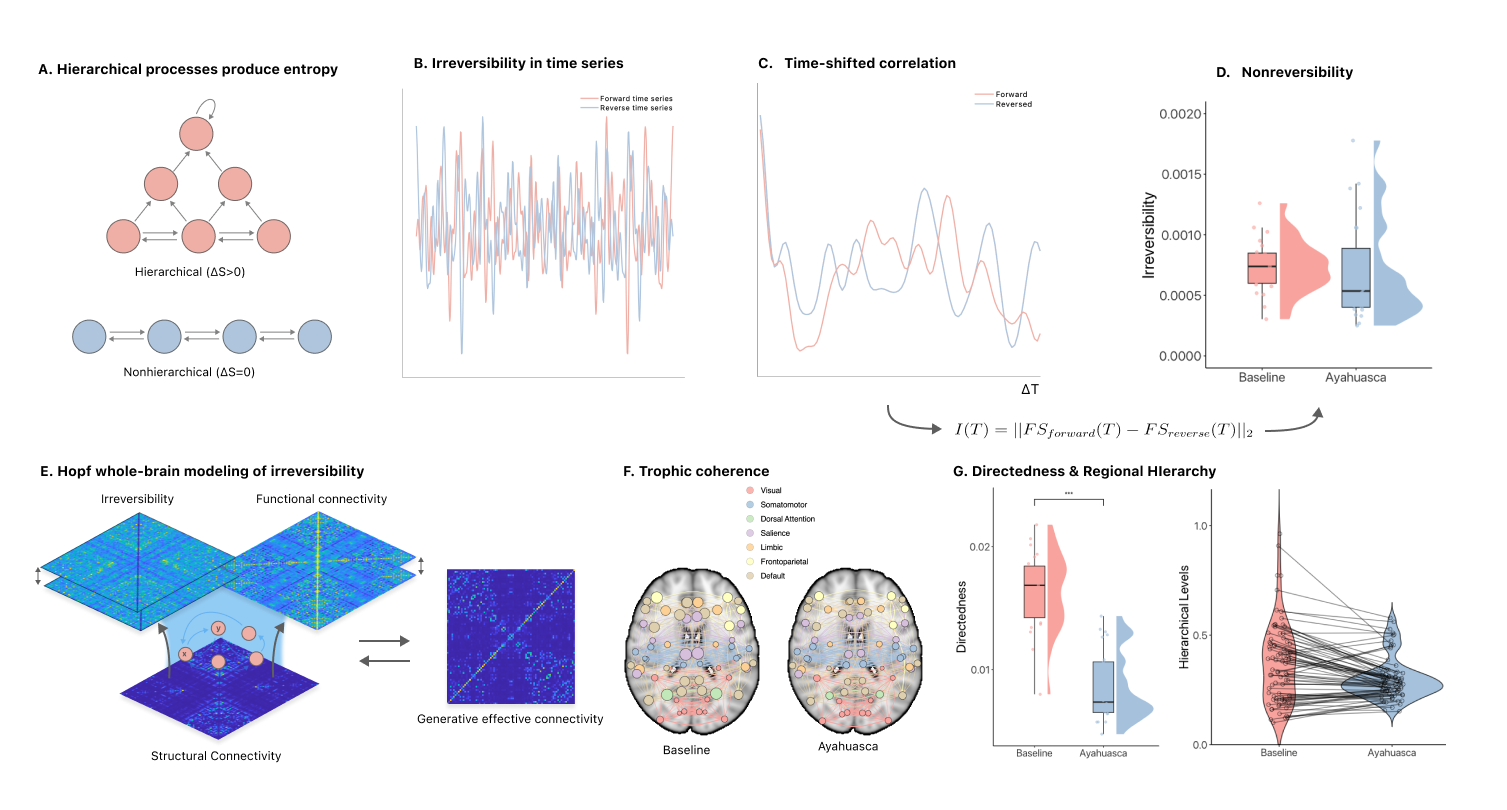
\includegraphics[width=\textwidth]{images/Figure 1.png}
    \caption[Trophic coherence provides causal insights into
the functional hierarchical organization of the brain on drugs]{Trophic coherence provides causal insights into
the functional hierarchical organization of the brain on psychedelics and cannabis. The
figure shows the overall methodological flow presented in this present
study. (A). Participants in three datasets (ayahuasca, DMT, chronic and occasional use of cannabis) were scanned during peak experiences with fMRI (see Methods for acquisition details). BOLD timeseries were extracted after preprocessing. 
(B). Hierarchical processes produce entropy via
irreversible flow of information. Non-hierarchical systems are in
detailed balance and fully reversible, whereas hierarchical systems
break detailed balance. Irreversibility in time-series can be extracted from the
asymmetry between forward and reversed timeseries, shifted in time.
(C) Irreversibility is computed as mutual information, represented by the
absolute quadratic difference, between the time-shifted pairwise
correlation of the forward and reversed timeseries, across all voxels in
the brain. Irreversibility is given by the IR matrix, and hierarchy is
represented as the variability of asymmetry in underlying causal
interactions for each participant in each condition (see Methods).
(D). The irreversibility and structural
anatomical connectivity derived from diffusion tensor imaging (DTI) are used to fit a whole-brain Hopf model, estimating the effective connectivity of irreversibility (see Methods).
(E). The hierarchical influence of each
region in the brain over others (left, right) and the overall trophic coherence, or directedness, of
hierarchical organization (middle), are given through trophic coherence (see Methods). Wilcoxon signed-rank test, middle panel. Non-parametric
two-sample permutation-based test followed by False Discovery Rate,
right panel. (* p\textless0.05; ** p\textless0.01; *** p\textless0.001)}
    \label{fig:overview}
\end{figure}

\section{Irreversibility}
To determine the effects of ayahuasca, DMT, and
cannabis on BOLD fMRI-derived brain hierarchy, 
we first computed irreversibility, an estimate of
production entropy. Irreversibility provides a quantification of how the environment is differentially
driving brain dynamics out of equilibrium depending on the underlying
brain state \parencite{Deco2022,Kringelbach2023}. This is especially relevant within the
context of the psychedelic experience and associated changes in brain
dynamics from long-term use as psychedelics are known to modulate
sensitivity to the environment and extrinsic stimuli, which is
consistent with the role of serotonergic neurotransmission in
environmental sensitivity regulation \parencite{Branchi2011,Carhart-Harris2017}.

We analyzed irreversibility over an 8-minute period after the injection
of DMT or placebo, \textasciitilde12-minute period 1h after the oral
ingestion of ayahuasca, and 6-minute period beginning 15 minutes after
inhalation of cannabis or placebo. The ideal time delay was calculated by finding the value that most effectively discriminated between conditions (see Figure \ref{fig:tau}). Compared
with baseline and placebo conditions, irreversibility was found to be
reduced significantly for DMT (Z=2.79, d = 1.05 [0.32 1.77], p = 0.0052)  and chronic use of
cannabis (Z=2.79, d= 1.05 [0.32 1.77], p = 0.0052) across the whole brain (Figure \ref{fig:ir}a).
Non-significant trends toward decrease were found for ayahuasca (p = 0.41) and
occasional use of cannabis (p = 0.14). A measurement of hierarchy was derived from
the standard deviation of irreversibility for each subject (Figure \ref{fig:ir}b). These results suggest that DMT and chronic
use of cannabis decrease the weight of extrinsic dynamics, or the
environment, on intrinsic brain dynamics.

\begin{figure}[h!]
    \centering
    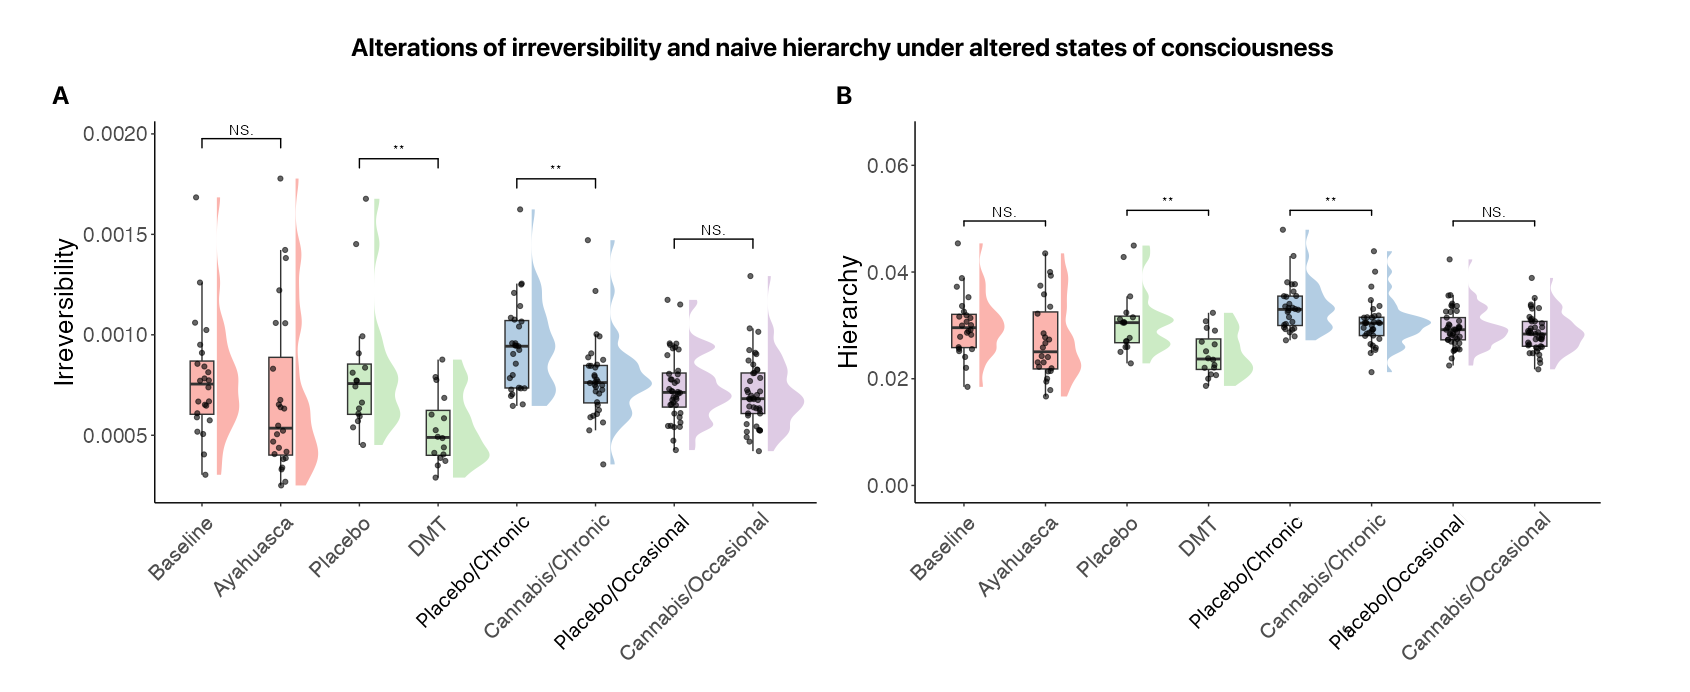
\includegraphics[width=\textwidth]{images/Figure 2_ Nonreversibility.png}
    \caption[Irreversibility and hierarchy of global brain dynamics under
different substances.]{Irreversibility and hierarchy of global brain dynamics under
different substances. (A) Global irreversibility across 80
regions of the DBS80 for ayahuasca, DMT, chronic use of cannabis, and
occasional use of cannabis. Significant decreases,
as evaluated by non-parametric Wilcoxon signed-rank test, were found for DMT>Placebo (Z=2.79, d = 1.05 [0.32 1.77], p = 0.0052) and the
chronic use of cannabis (Z=2.79, d= 1.05 [0.32 1.77], p = 0.0052) , but not occasional use (p = 0.14). A nonsignificant trends
toward decrease in irreversibility was found for ayahuasca (p = 0.41) (B) Similar results were found for
a simple measure of hierarchy, defined as the standard deviation of
irreversibility. Significant differences were found for the change in
irreversibility from placebo to DMT (Z = 2.74, d = 1.14 [0.40 1.86], p = 0.0061), and from baseline to acute cannabis
experience for chronic users (Z = 2.32, d = 0.69 [0.17 1.20], p = 0.02). Nonsignificant decreases in hierarchy were
found for ayahuasca (p = 0.15) and occasional users of cannabis (p = 0.21). (* p\textless0.05;
** p\textless0.01; *** p\textless0.001).}
    \label{fig:ir}
\end{figure}

\section{Trophic coherence of altered states of consciousness}
This first-pass analysis showed that changes in irreversibility, an indirect measure of hierarchy,
are present under both psychedelic and cannabis conditions. We further
examined changes in hierarchy by analyzing the effective connectivity
through whole-brain modelling with generative effective connectivity (GEC) \parencite{Kringelbach2023}. Irreversibility provides information about whether or not hierarchical, or directional, information flow exists between two regions, but does not inform one of which direction that information is moving in. The framework presented here,
first implemented by \textcite{Deco2022}, is less
computationally expensive than alternatives including direct estimation
of the entropy rate through methods like transfer entropy for measuring
Granger causality, and deep learning models \parencite{Deco2021a,Lynn2021,SanzPerl2021,Seif2021}.
Furthermore, this framework has been shown to estimate precise
signatures of different brain states in both electrocorticography (ECoG) data
from non-human primates, including awake, deep sleep, and anesthesia, as
well as differentiating between tasks, rest, and movie-watching in
humans \parencite{Deco2022,Kringelbach2023}.

The model-free quantification of the level of irreversibility is used as
a basis by which to fit a causal, mechanistic whole-brain model, which
provides the effective weighting of the existing structural connectivity
as derived from diffusion tensor imaging \parencite{Friston2003}.
Here, we derived anatomical connectivity from the Human Connectome
Project with 32 participants. This presents a limitation, as
anatomical connectivity is known to vary across individuals and may
result in a less accurate fit to functional connectivity and
irreversibility \parencite{Mueller2013}. The whole-brain model adapts the
strength of existing anatomical connectivity by altering conductance
value parameters in order to optimize connectivity. Iterative estimation of the GEC with
pseudo-gradient descent optimization allows for fitting to the
empirical irreversibility covariance matrix, minimizing the mean-squared
error between empirical and simulated functional connectivity matrices
and the irreversibility covariance matrices. This model, in turn, allows
for evaluation of the generative mechanisms creating hierarchy within
conditions and, importantly, the hierarchical reconfiguration between conditions. A Hopf oscillator model was used as it has previously been shown it
provides the best fit \parencite{Deco2017c, Deco2019a,Deco2017b, Kringelbach2023}. Deviations between empirical and optimized, convergent
simulated functional connectivity and respective covariance matrices are
available in Supplemental Figure \ref{fig:fits}.

The extent to which one region orchestrates the activity of others is
evaluated through summation of the in-degree and out-degree across each region in the brain. As can be seen in Figure \ref{fig:gecrender}, this measure of orchestration varies significantly across conditions. Under the long-term users of ayahuasca, orchestration was found to be most significant in the bilateral pre- and post-central, insula, and superior temporal, as well as the superior frontal gyrus. Under DMT, the insula was less well-connected, though bilateral precuneus became more connected. Under chronic use of cannabis, significant orchestrators were the bilateral isthmus cingulate and rostral anterior cingulate, as well as the bilateral insula. Similarly, bilateral isthmus cingulate and rostral anterior cingulate were primary orchestrators of functional organization under the occasional use of cannabis, as well as the bilateral insula. To complement the analysis of information flow between different regions
captured by the GEC matrix under altered states of consciousness, we
decomposed all brain regions into their canonical resting-state networks
and evaluated changes between baseline or placebo and
drug conditions on orchestration, characterized by the sum of
the in-degree and out-degree, or incoming and outgoing information, from
each network \parencite{Yeo2011}. Figure \ref{fig:gecrender}c details the modulation of
resting-state network orchestration by ayahuasca, DMT, and cannabis.

Regional and network-level orchestration provides information about connectivity changes, but the degree to which a region orchestrates global brain activity is not directly a measure of hierarchy. To better examine the effects of chronic and occasional use of
psychedelics and cannabis on the functional, hierarchical organization
of the brain, we applied trophic coherence to the effective connectivity
derived from the GEC, utilizing the degree of orchestration for each region. Trophic coherence, which we call directedness to differentiate from the method itself, is primarily a measure of how neatly nodes
in a network fall into distinct levels, which is analyzed by the
standard deviation of the distribution of height differences along edges \parencite{Johnson2014,MacKay2020}. The measure was first
applied to ecological food webs in an attempt to better understand the
stability of networks, but it can be applied to any directed network. Previously, it was used to model the coherence of social systems, including dictatorships, military regimes, and anarchy, which found that rigid, hierarchical social systems tend to have higher directedness than democracies or anarchy \parencite{Pilgrim2020}. That is, a higher directedness is associated with a more rigid, stratified network structure.
Here, we consider the effective connectivity of the brain as a directed network, where the degree to which a region orchestrates activity assigns it a trophic, or hierarchical, level that describes its influence over the brain. It is then possible to query the directedness of the network. Networks which display high directedness are clearly defined with regard to each nodes influence over others and are highly stratified. The corollary is that networks with low directedness are highly disordered and lack clearly defined influence relations.

\begin{figure}[h]
    \centering
    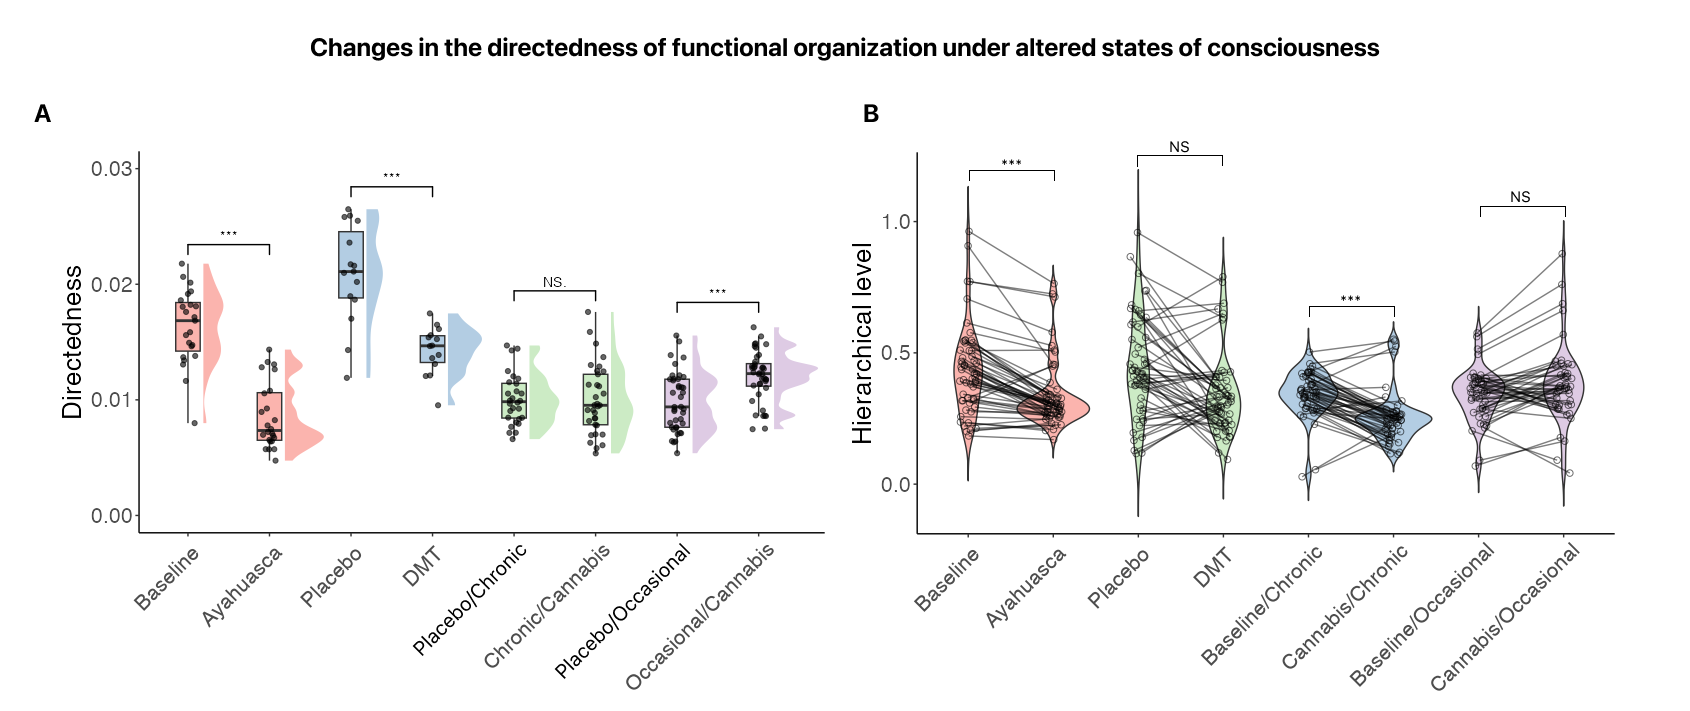
\includegraphics[width=\textwidth]{images/Figure 3_ Trophic coherence.png}
    \caption[Changes in directedness of hierarchical organization under altered state s of consciousness]{Changes in the directedness of functional organization under altered
states of consciousness. (A) Changes in directedness of the
effective connectivity between baseline and placebo and drug conditions.
Compared with baseline, directedness under ayahuasca (t = -8.92, d = 2.50 [1.73 3.26], p = 2.015e-11) and DMT significantly
decreased (d = 0.82 [0.10 1.54], p = 0.010). Interestingly, baseline directedness was much higher for participants in the DMT dataset. Nonsignificant trend
toward decrease was found for the chronic use of cannabis (p = 0.52), while a
significant increase in directedness was found for the occasional use of
cannabis (Z = -3.83, d = -0.91 [-1.36 -0.45], p = 1.28e-4). (B) Changes in trophic levels
after 10,000 iteration non-parametric permutation testing (threshold =
0.01, FDR correction threshold = 0.2). Under ayahuasca, most regions tend to decrease in hierarchical level, while both trends exist for DMT.}
    \label{fig:TC}
\end{figure}

We first analyzed the changes in directedness of the functional
organization of the brain under different states of consciousness, as
well as changes in the individual trophic levels for each region in
the brain from baseline or placebo to drug condition. In Figure \ref{fig:TC}a, it
can be seen that directedness, a direct measure of hierarchical organization,
significantly decreases under ayahuasca (t = -8.92, d = 2.50 [1.73 3.26], p = 2.015e-11) and DMT (d = 0.82 [0.10 1.54], p = 0.010).
In contrast, the occasional use of cannabis resulted in a significant
increase in the directedness of the brain's functional hierarchical
organization (Z = -3.83, d = -0.91 [-1.36 -0.45], p = 1.28e-4), while chronic use of cannabis had no
effect (p = 0.52), possibly due to tolerance \parencite{Ramaekers2022}. Due to differences in study design,
fMRI equipment, and acquisition and preprocessing techniques it is not
possible to make statistical comparisons against conditions. However, we
were uniquely positioned to make inferences about the nature of chronic
and occasional use of psychedelics and cannabis. We also examined changes in hierarchical levels
for each of 80 regions with a 10,000 iteration non-parametric permutation test, followed
by a second permutation test between mean hierarchical level changes across regions between conditions.
In Figure \ref{fig:TC}b, alterations in the hierarchical levels within regions across conditions can be seen. Alterations in directedness
can be considered as a change in the variance of hierarchical levels across conditions.
While directedness decreased significantly for DMT, hierarchical levels varied with regard
to their change in influence. For ayahuasca and occasional use of cannabis, most levels decreased greatly, with the exception
of a few at the bottom of the hierarchy. A similar pattern was seen for the chronic and occasional use of cannabis, where
regions at the bottom and top of the hierarchy tended to increase in influence.

While the measure of orchestration provides a measure of the connectedness of regions, it does not \textit{a priori}
necessitate alterations in hierarchy. 
Trophic coherence, in contrast, provides direct access to
examining alterations in the functional hierarchical organization of the brain. Figure 
\ref{fig:tcrender} details the trophic levels which describe 
the degree of influence a brain region holds for each 
condition. As can be seen in Figure \ref{fig:tcrender}a, 
variability in trophic levels is visually distinct for the chronic and 
occasional use of cannabis versus ayahuasca and DMT. Considerable variability under cannabis for occasional users 
differs from the DMT state, whose variability is similar to 
ayahuasca. These results suggest that tolerance and chronicity 
play a different role in the changes in functional organization 
underlying disparate
altered states of consciousness. 

\begin{figure}[h!]
    \centering
    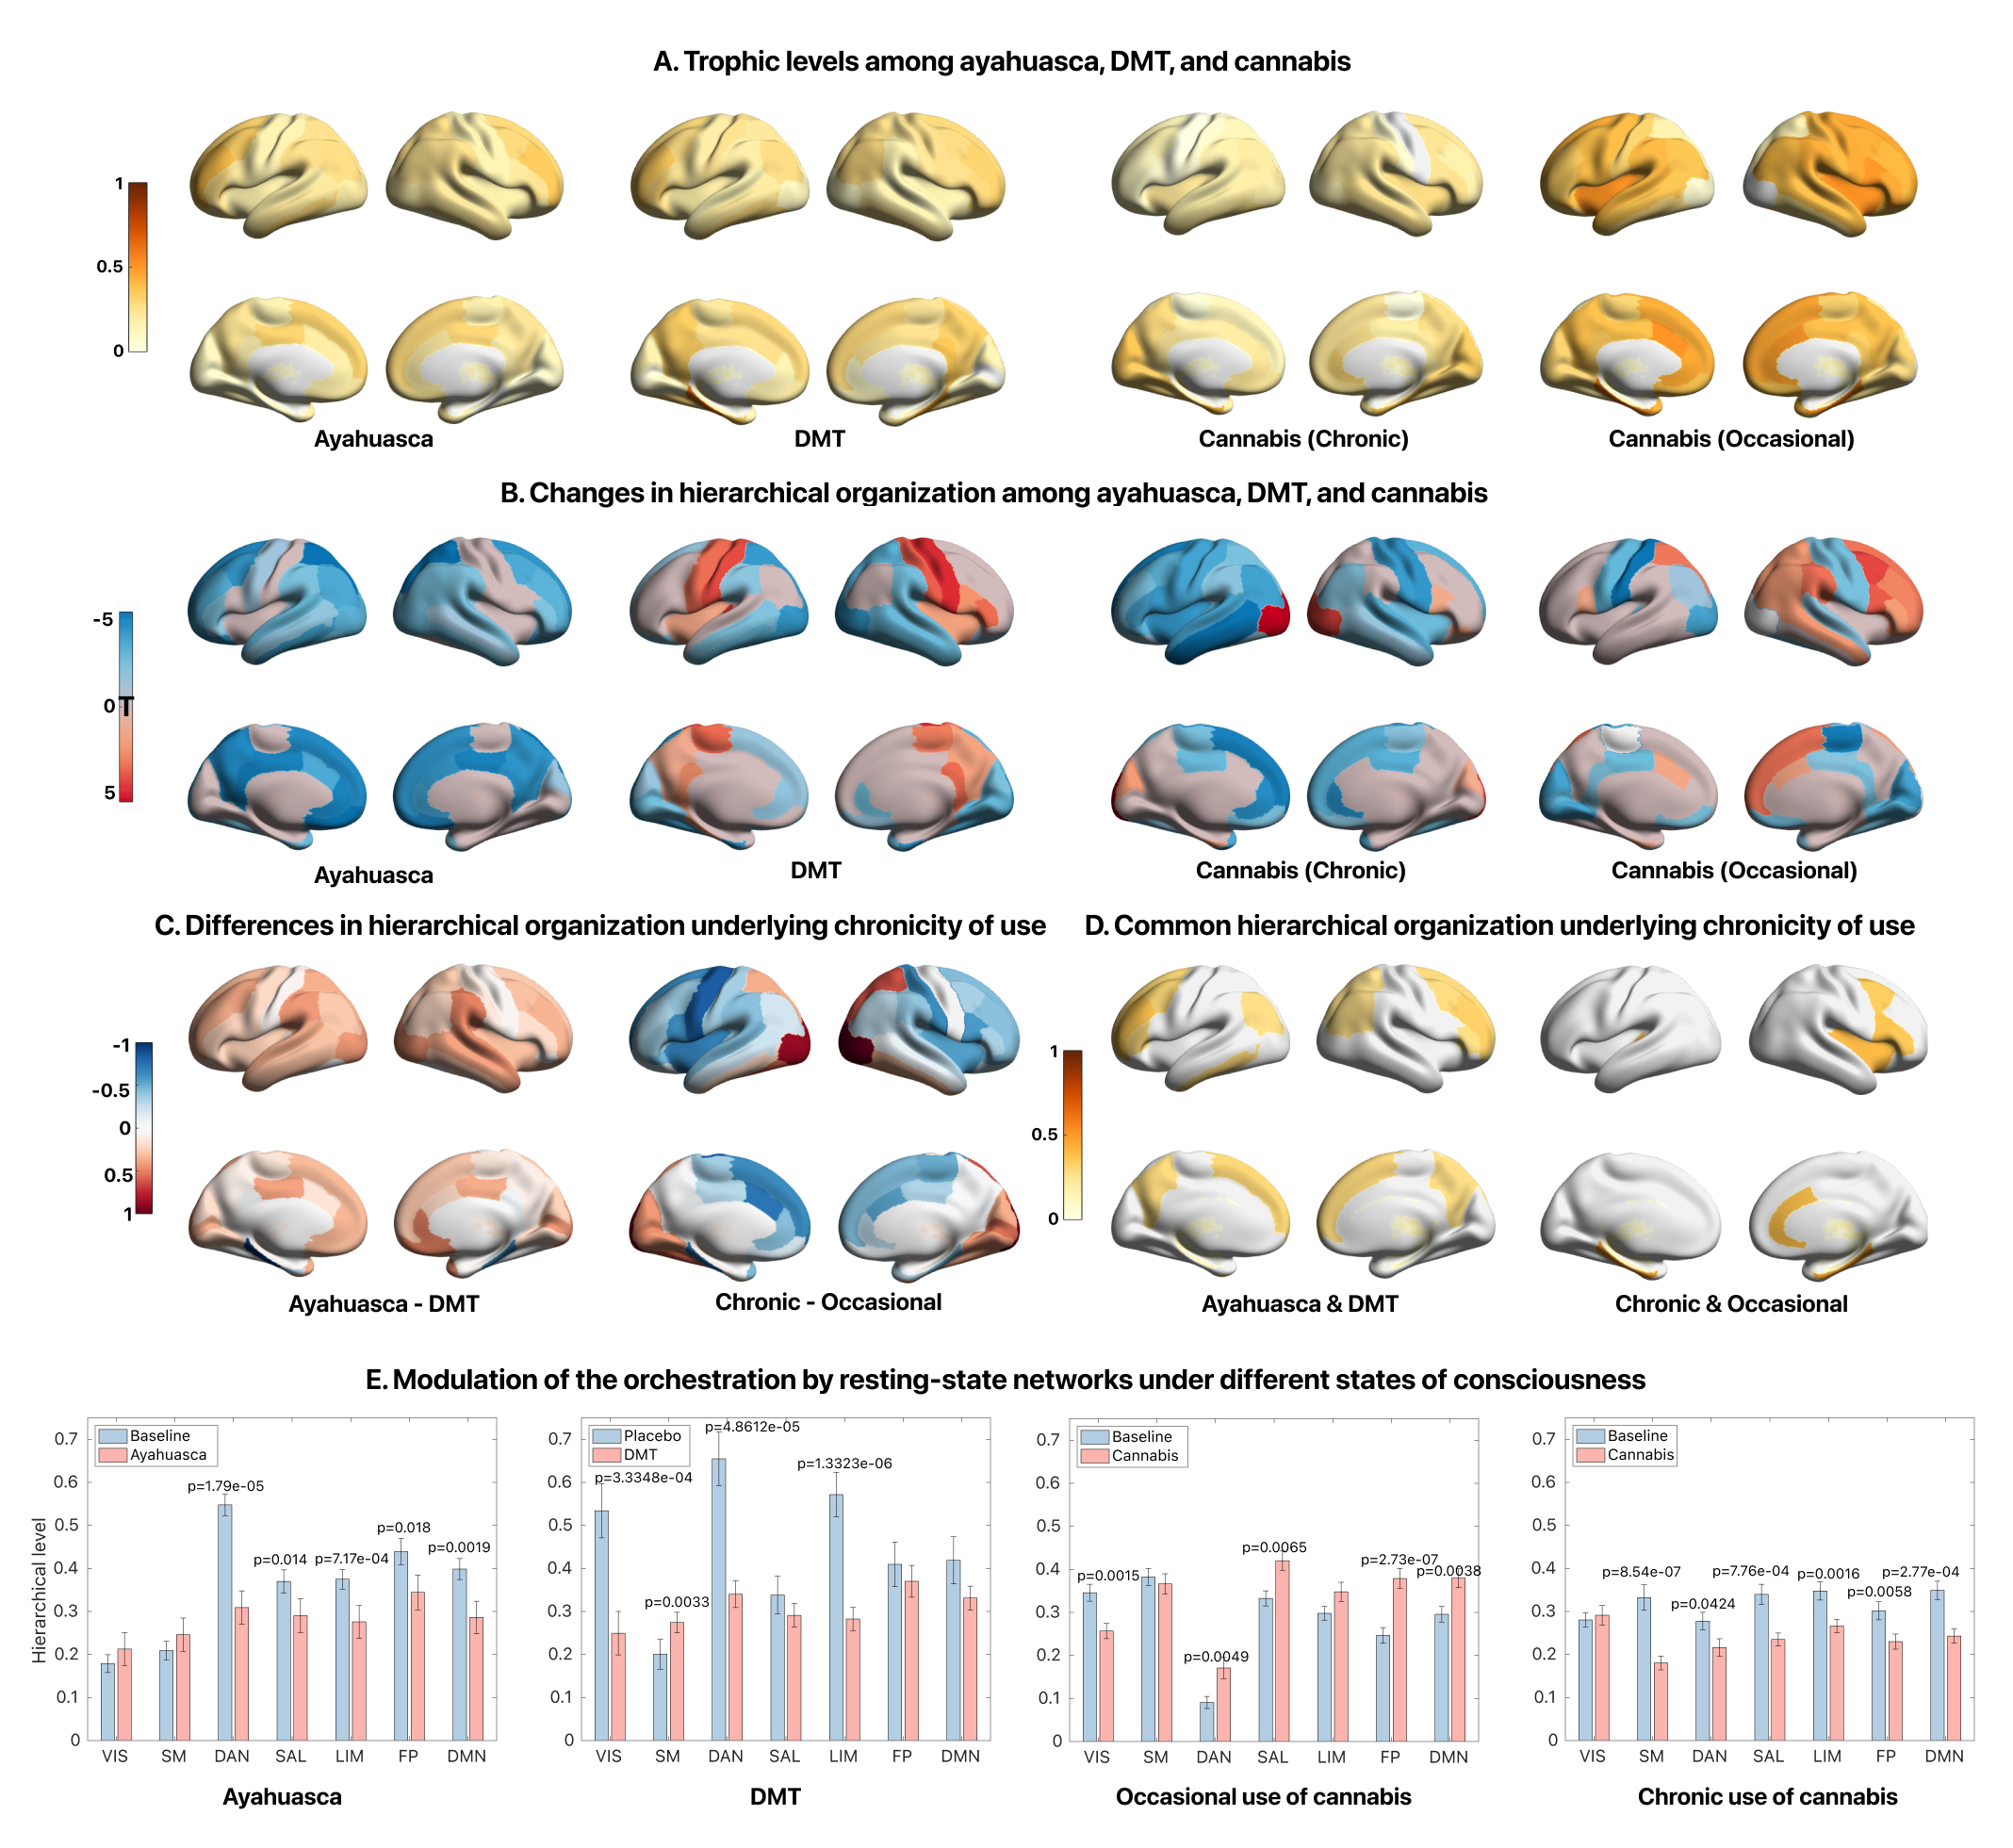
\includegraphics[width=\textwidth]{images/Figure 4_ HL.png}
    \caption[Changes in regional hierarchy orchestrating altered states and their common architecture.]{Changes in
the regional hierarchy orchestrating altered states and their common
hierarchical architecture. (A) Regional hierarchy in acute ayahuasca, DMT,
and cannabis in chronic and occasional users. Significant variability
can be seen for occasional users on cannabis, but not for ayahuasca,
DMT, or cannabis in chronic users. (B) Changes in regional hierarchy
from baseline or placebo to drug condition. Non-parametric 10,000 permutation 
testing with FDR correction identified significant regions. Non-significant regions are shaded grey. (C) Differences in regional hierarchy underlying chronicity of drug use in acute conditions.
Ayahuasca resulted in generally higher regional hierarchy across the cortex than DMT
. With cannabis, occasional use resulted in stronger hierarchy than in chronic use,
except for the occipital cortex. (D) Common regional hierarchy underlying chronicity of drug use in acute conditions. The top 25\% regions in the hierarchy were examined for each drug condition and we found the intersection between
the psychedelics and between cannabis conditions.(E) Modulation of resting-state network hierarchy. Significant decreases (5,000 iteration non-parametric permutation testing, FDR corrected) were found for ayahuasca, DMT, and chronic use of cannabis. Variability in regional hierarchy was found for occasional use of cannabis.}
\label{fig:tcrender}
\end{figure}

We examined changes from baseline or placebo for each condition 
through individual, 10,000 iteration non-parametric permutation 
tests for each region across each condition. It can be seen 
that unlike ayahuasca, DMT resulted in considerable increases in 
bilateral pre- and post-central trophic levels, as well as in 
the bilateral precuneus, paracentral, and isthmus cingulate 
(Figure \ref{fig:tcrender}b). The largest increases 
and decreases in trophic levels for each condition provide 
additional information about the nature of these altered 
states. Interestingly, increases in trophic levels were found 
for subcortical structures under ayahuasca, including the right 
putamen (P < 0.01, FDR corrected) and left globus pallidus externus, not rendered here (P 
< 0.01, FDR corrected). Decreases were seen in 
bilateral superior parietal, left medial orbitofrontal, left 
isthmus cingulate, and left posterior cingulate, consistent 
with previous results \parencite{Timmermann2019,Carhart-Harris2016}. For DMT, increases were found in left and right 
pre-central, left transverse temporal, and left and right post-central (P < 0.01, FDR corrected). Under the chronic 
use of cannabis, decreases in trophic level were seen all 
across the brain, except in left and right medial and lateral 
occipital cortex, left and right thalamus, and right globus 
pallidus internus (P < 0.01, FDR corrected). Decreases 
were found in left middle temporal, left inferior temporal 
cortex, left superior frontal cortex, and the left and right 
rostral anterior cingulate cortices (P < 0.01, FDR 
corrected). For the occasional use of cannabis, increases were 
found in the right subthalamic nucleus, right caudal middle 
frontal, right pars opercularis, right supramarginal, and right 
superior frontal (P < 0.01, FDR corrected). Decreases 
in regional hierarchy were found in the right lateral 
occipital, left and right paracentral, left post-central, and 
right pericalcerine (P < 0.01, FDR corrected). 

We then examined differences in regional hierarchy between acute occasional and chronic use contrasts (Figure \ref{fig:tcrender}c). Ayahuasca generally had higher regional hierarchy across the cortex than did DMT -- in particular, left rostral anterior cingulate cortex and right supramarginal. For Chronic>Occasional, it was found that cannabis in occasional users induced considerably higher regional hierarchy than in chronic users, except in the medial and lateral left and right occipital cortices and superior parietal cortices. After finding differences between conditions, we sought to understand common effects of psychedelics and cannabis across the chronicity of use (Figure \ref{fig:tcrender}d). We took the top 50\% of regions in the hierarchy and evaluated the intersection between them. For ayahuasca and DMT, these common influential regions were in the frontal cortex, as well as left and right superior parietal cortices, superior frontal cortices, and precuneus. For cannabis in chronic and occasional users, these common regions were the right insula, pars opercularis, pars triangularis, and caudal middle frontal, as well as the left anterior cingulate cortex.

\begin{figure}[h!]
    \centering
    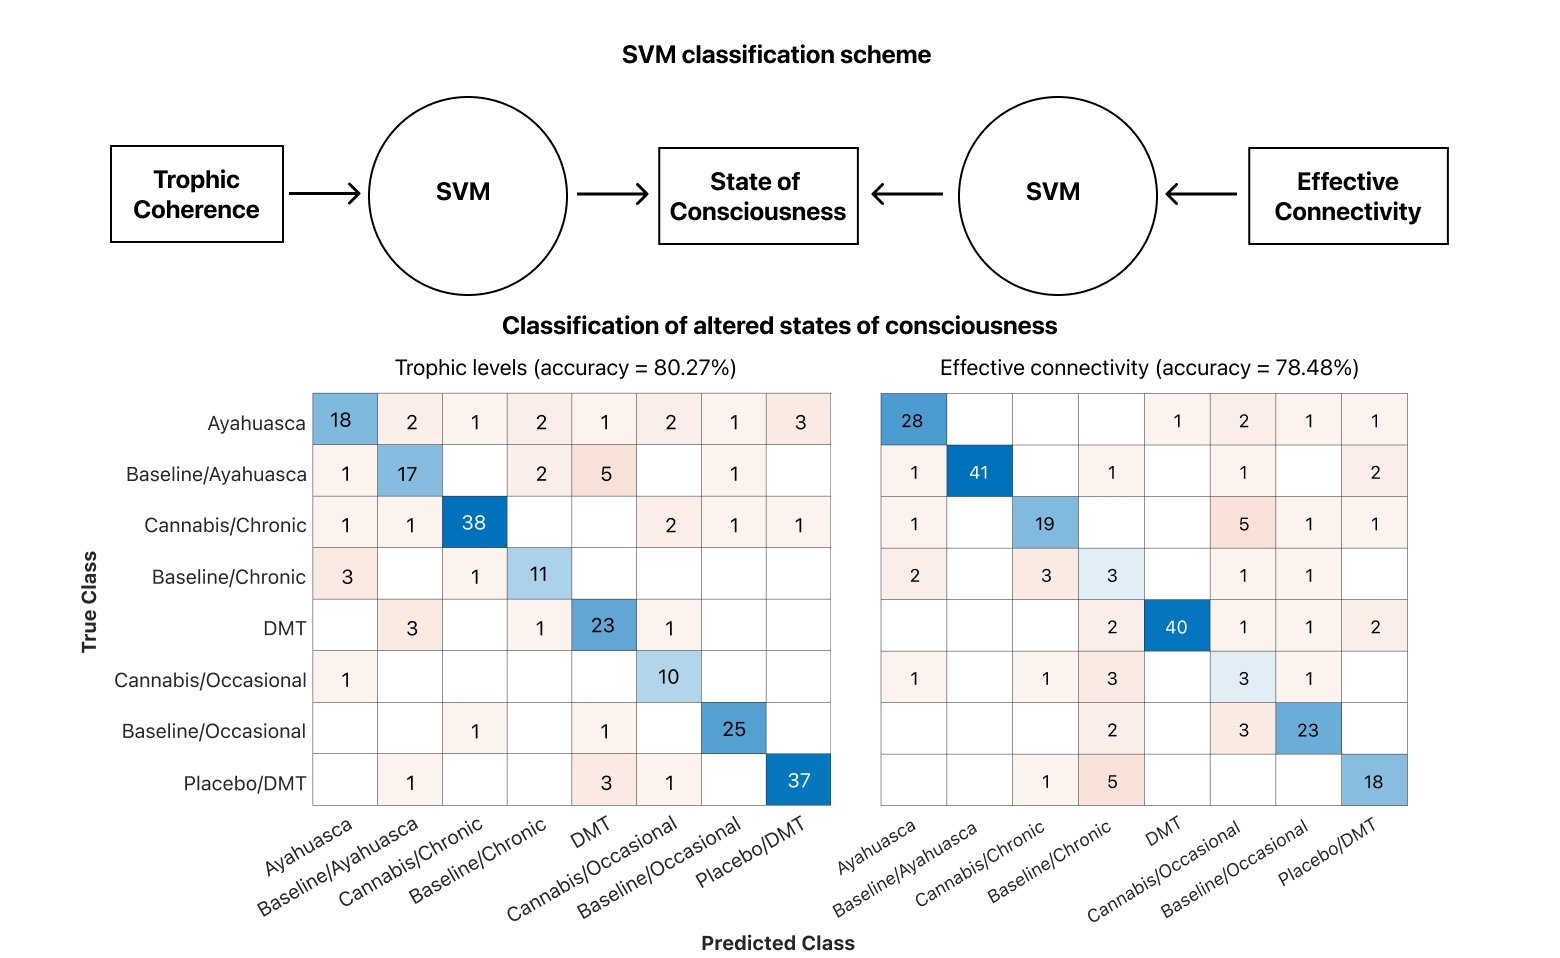
\includegraphics[width=\textwidth]{images/Figure 5 SVM.png}
    \caption[Trophic coherence
is an equivalently performing, simpler discriminator of states of consciousness than
effective connectivity.]{Trophic coherence
is an equivalently performing, simpler discriminator of states of consciousness than
effective connectivity. Figure shows the confusion matrix of the
classification performance (across 5-fold k-fold cross-validation). As
can be seen, the trophic coherence is an equal predictor
of the conscious state condition than effective connectivity (the GEC).
The average performance for trophic coherence is 80.27\%, while the
performance for effective connectivity is slightly lower
(78.48\%).}
    \label{fig:svm}
\end{figure}

To explore changes in the functional integrity of resting-state networks after the administration of psychedelics, we decomposed trophic levels for each region into the resting-state network most associated with that region for changes in trophic level from baseline. Figure \ref{fig:tcrender}e shows the alterations in resting-state network hierarchical influence after the administration of ayahuasca, DMT, and the chronic or occasional use of cannabis. Non-parametric, 10,000 iteration permutation-based hypothesis testing ($\alpha = 0.01$) was followed by FDR correction ($q=0.2$). Significant decreases were seen for ayahuasca and DMT in the dorsal attention and limbic networks, while ayahuasca also significantly decreased the influence of the salience, frontoparietal, and default mode networks (P < 0.05, FDR corrected). DMT, on the other hand, resulted in significant decreases in the visual network and increases in the somatomotor networks (P < 0.05, FDR corrected). Similarly, occasional use of cannabis saw decreases in the visual network, but increased network hierarchy in the dorsal attention, salience, frontoparietal, and default mode networks (P < 0.05, FDR corrected). Lastly, decreases were found across all resting-state networks but the visual network for the chronic use of cannabis (P < 0.05, FDR corrected). Interestingly, ayahuasca induced a non-significant increase in both visual and somatomotor networks, consistent with the idea of a disinhibition of unimodal sensory networks under psychedelics. It is quite a surprise that the visual network hierarchy was significantly higher in resting-state than on DMT.

\begin{figure}[h!]
    \centering
    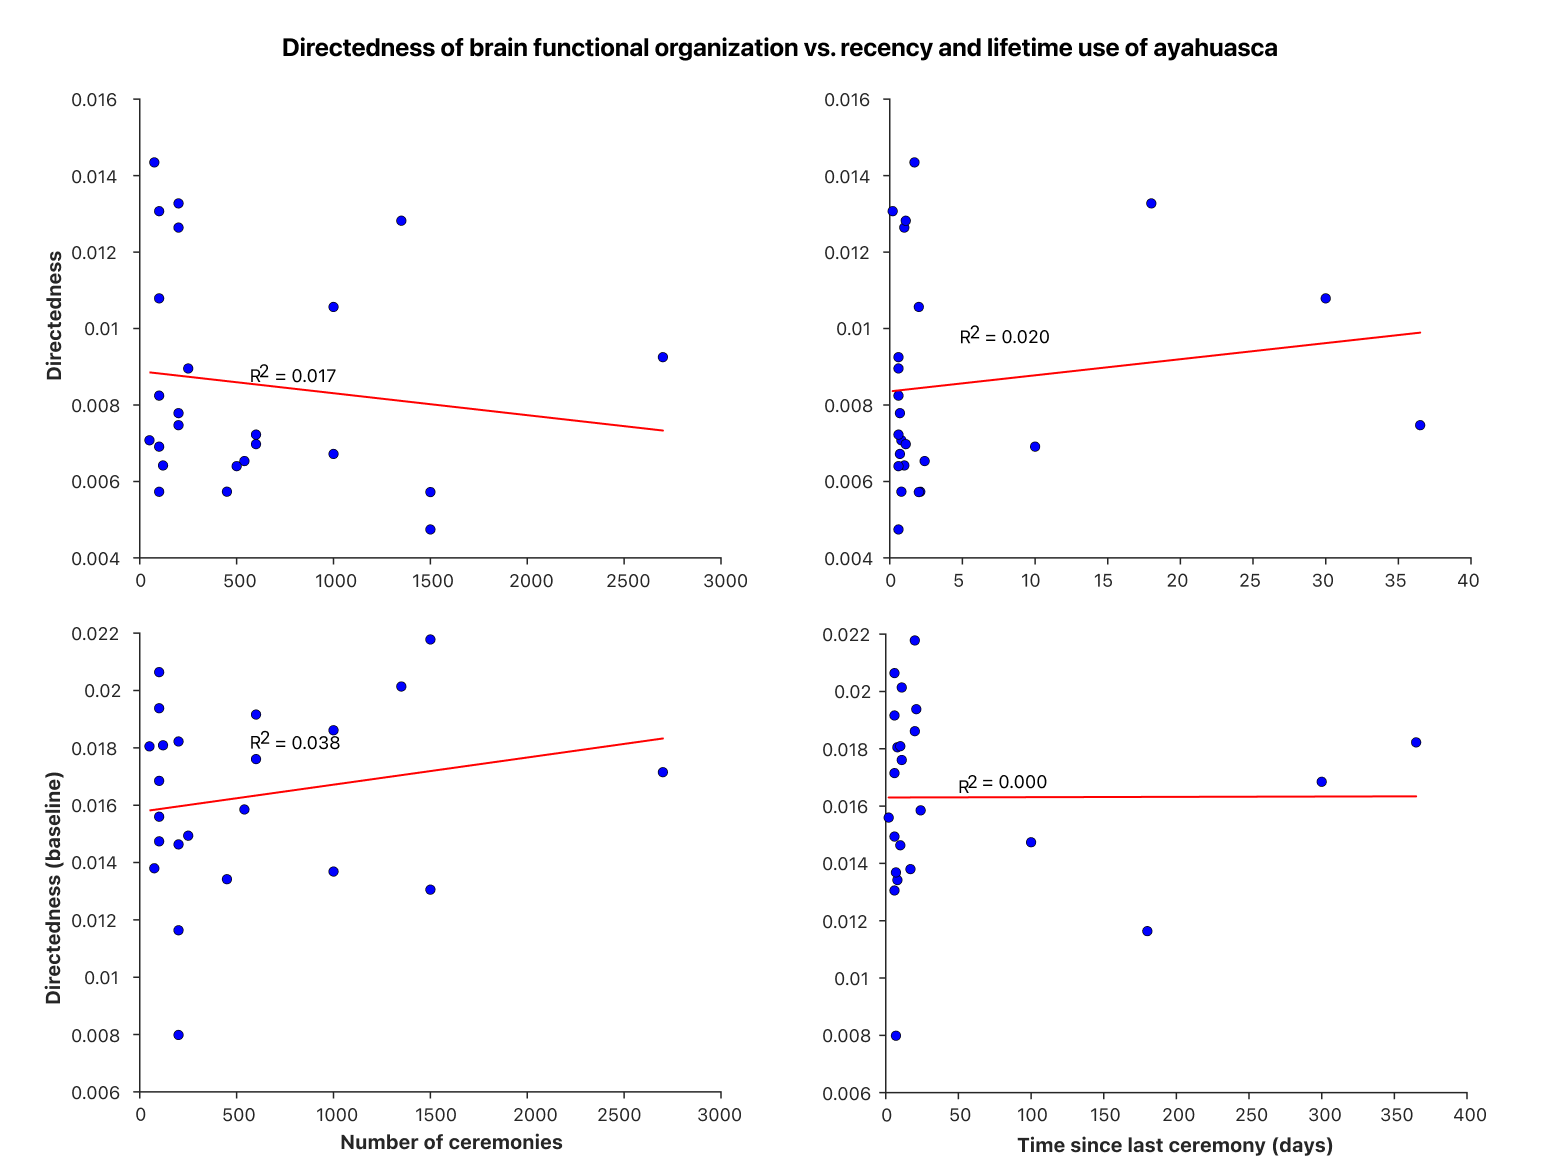
\includegraphics[width=\textwidth]{images/Figure 6_ Correlations between recency.png}
    \caption[Directedness of brain functional organization vs. lifetime use and recency of use.]{Directedness of brain functional organization vs.~lifetime use of
ayahuasca and recency of use. Linear mixed effect models were fit with
directedness (pre- or post-ayahuasca) as the variable to be predicted,
lifetime use or recency as fixed effects, and dosage as a covariate.
Statistical significance was not found for any parameter. Post-ayahuasca
vs number of ceremonies (top-left panel) showed a downward trend with
regard to directedness, with weak correlation (\(R^2=0.017\), p = 0.85).
Post-ayahuasca vs.~time since last ceremony showed an upward trend with
weak correlation (\(R^2=0.020\), p = 0.73). Baseline measures of directedness
(bottom-left panel) showed opposite results against number of
ceremonies, where baseline directedness tended to be higher as the total
number of ceremonies for each participant increased (\(R^2=0.0038\), p = 0.99).
Baseline measures of directedness show no trend with time since last
ceremony (\(R^2=0.000\), p = 0.37).}
    \label{fig:corr}
\end{figure}

Developing a new framework for assessing the direct, causal interactions
orchestrating changes in the functional hierarchical organization of the
brain not only required the evaluation of how these measures compared
with irreversibility and the measure of orchestration of the GEC, but
also to understand whether regional hierarchy can better discriminate
between altered states of consciousness than effective connectivity
alone. We fit a support vector machine (SVM) as a classifier using
either the regional trophic levels or the effective connectivity matrix to
classify the state of consciousness across conditions. Figure \ref{fig:svm} shows
the classification scheme, as well as the confusion matrix
describing the accuracy of models (see Methods). It was found that regional hierarchy
predicted the drug or baseline/placebo condition with 80.27\% accuracy,
while the effective connectivity matrix predicted the condition with 78.48\% accuracy. Directedness, and the global measure of irreversibility are not suitable for this sort of classifier approach -- more features are needed, which is why we use either the subjects-by-region trophic level matrix, or the region-by-by-region irreversibility matrix. In this case, the trophic levels are considered to be less rich in terms of raw data, but the classifier is able to predict equally the state with a small increase in accuracy. Regional hierarchy derived by trophic coherence thus provides a
substantive and accurate dimensionality reduction of the network properties of the irreversibility matrix that captures the functional hierarchical
organization of the brain.

Lastly, we endeavored to better understand the relationship between lifetime use of\\ psychedelics, recency of use, and alterations in functional hierarchical organization. We modeled the linear relationship
between the directedness of networks and lifetime use or recency for
both baseline levels of directedness, as well as altered levels under
ayahuasca. In Figure \ref{fig:corr}, it can be seen that there do not appear to exist
any trends between these measures. Linear mixed-effect models were fit
with post- or pre-ayahuasca directedness as outcome and lifetime use, in
this case number of ayahuasca ceremonies, or recency of use (time since
last ceremony) as fixed effects with the dosage of ayahuasca
administered as a covariate. Despite regional and network-level hierarchy differences between ayahuasca and DMT, a tolerance effect over both short and long timescales does not appear to be present. It may be the case that hierarchical measures do not provide an accurate representation of changes in the brain resulting from long-term use of psychedelics. 

\chapter{Discussion}
This is the discussion.
%\include{chapters/references}



%next line adds the Bibliography to the contents page
%\addcontentsline{toc}{chapter}{Bibliography}
%uncomment next line to change bibliography name to references
%\renewcommand{\bibname}{References}
%\bibliographystyle{apacite}  %use the plain bibliography style
%\bibliography{refs}        %use a bibtex bibliography file refs.bib
\chapter{References}
\printbibliography[heading=none]

%now enable appendix numbering format and include any appendices
\appendix
\chapter{Supplemental Figures}

\begin{figure}
    \centering
    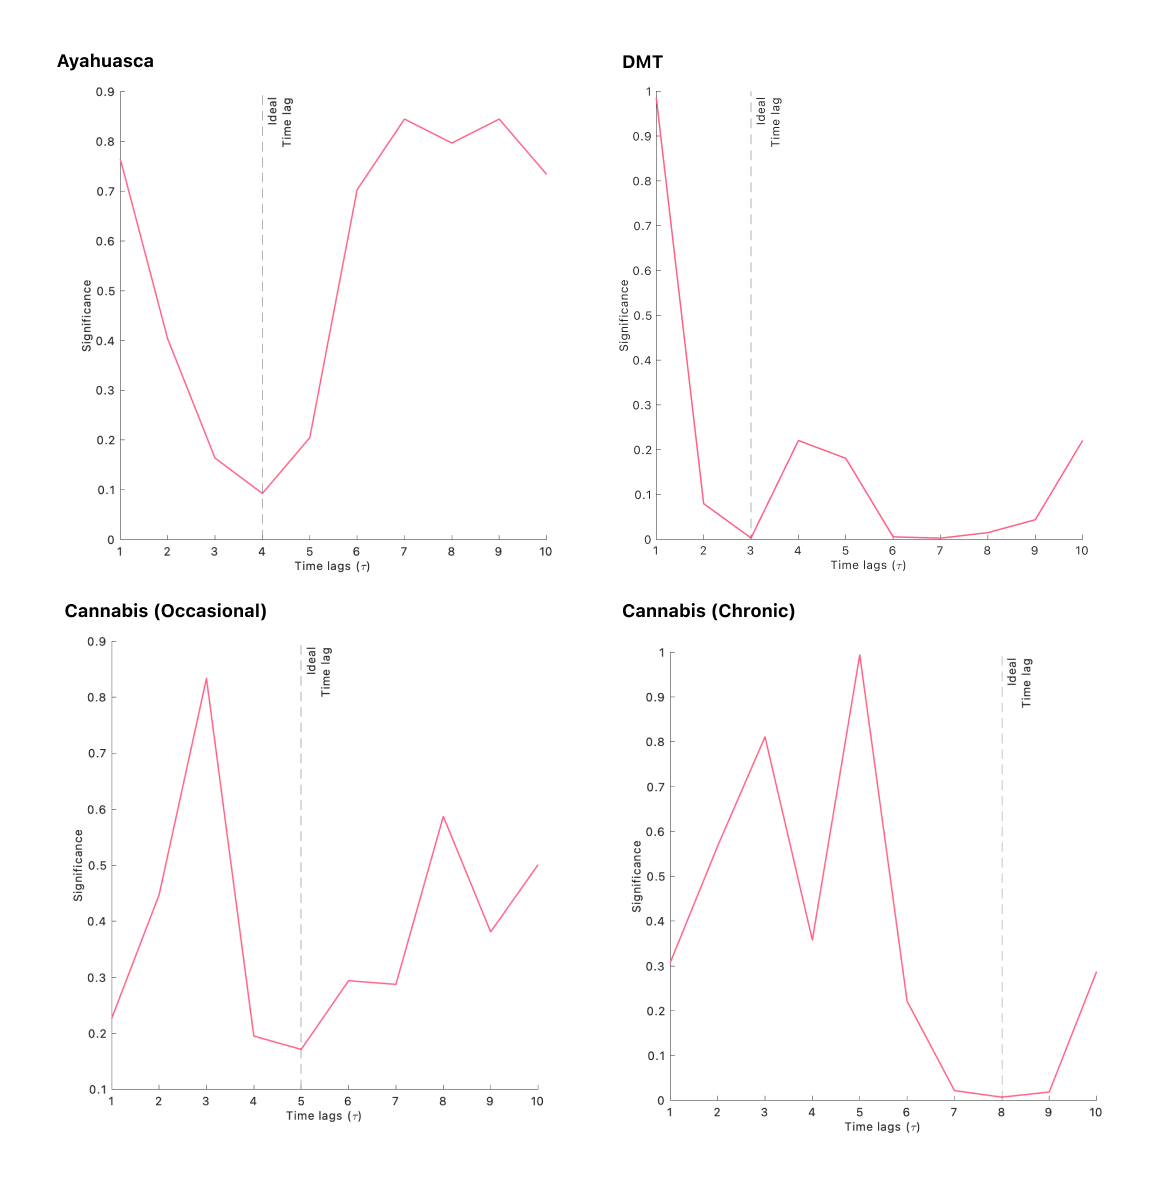
\includegraphics[width=\textwidth]{images/Appendix_ Tau Calculation.png}
    \caption[Establishing ideal $\tau$ for each condition.]{Evaluation of the ideal time-delay constant $\tau$ for each condition. Model-free irreversibility was calculated for Tau values 1 through 10 for each condition. For ayahuasca, occasional and chronic use of cannabis, a Wilcoxon rank-sum test was used to evaluate significance. The ideal Tau was determined as the most sensitive measure which best discriminates between baseline or placebo and drug conditions. For DMT, a mixed effects model was used in order to account for the pre-injection data as a covariate.}
    \label{fig:tau}
\end{figure}

\begin{figure}[h!]
    \centering
    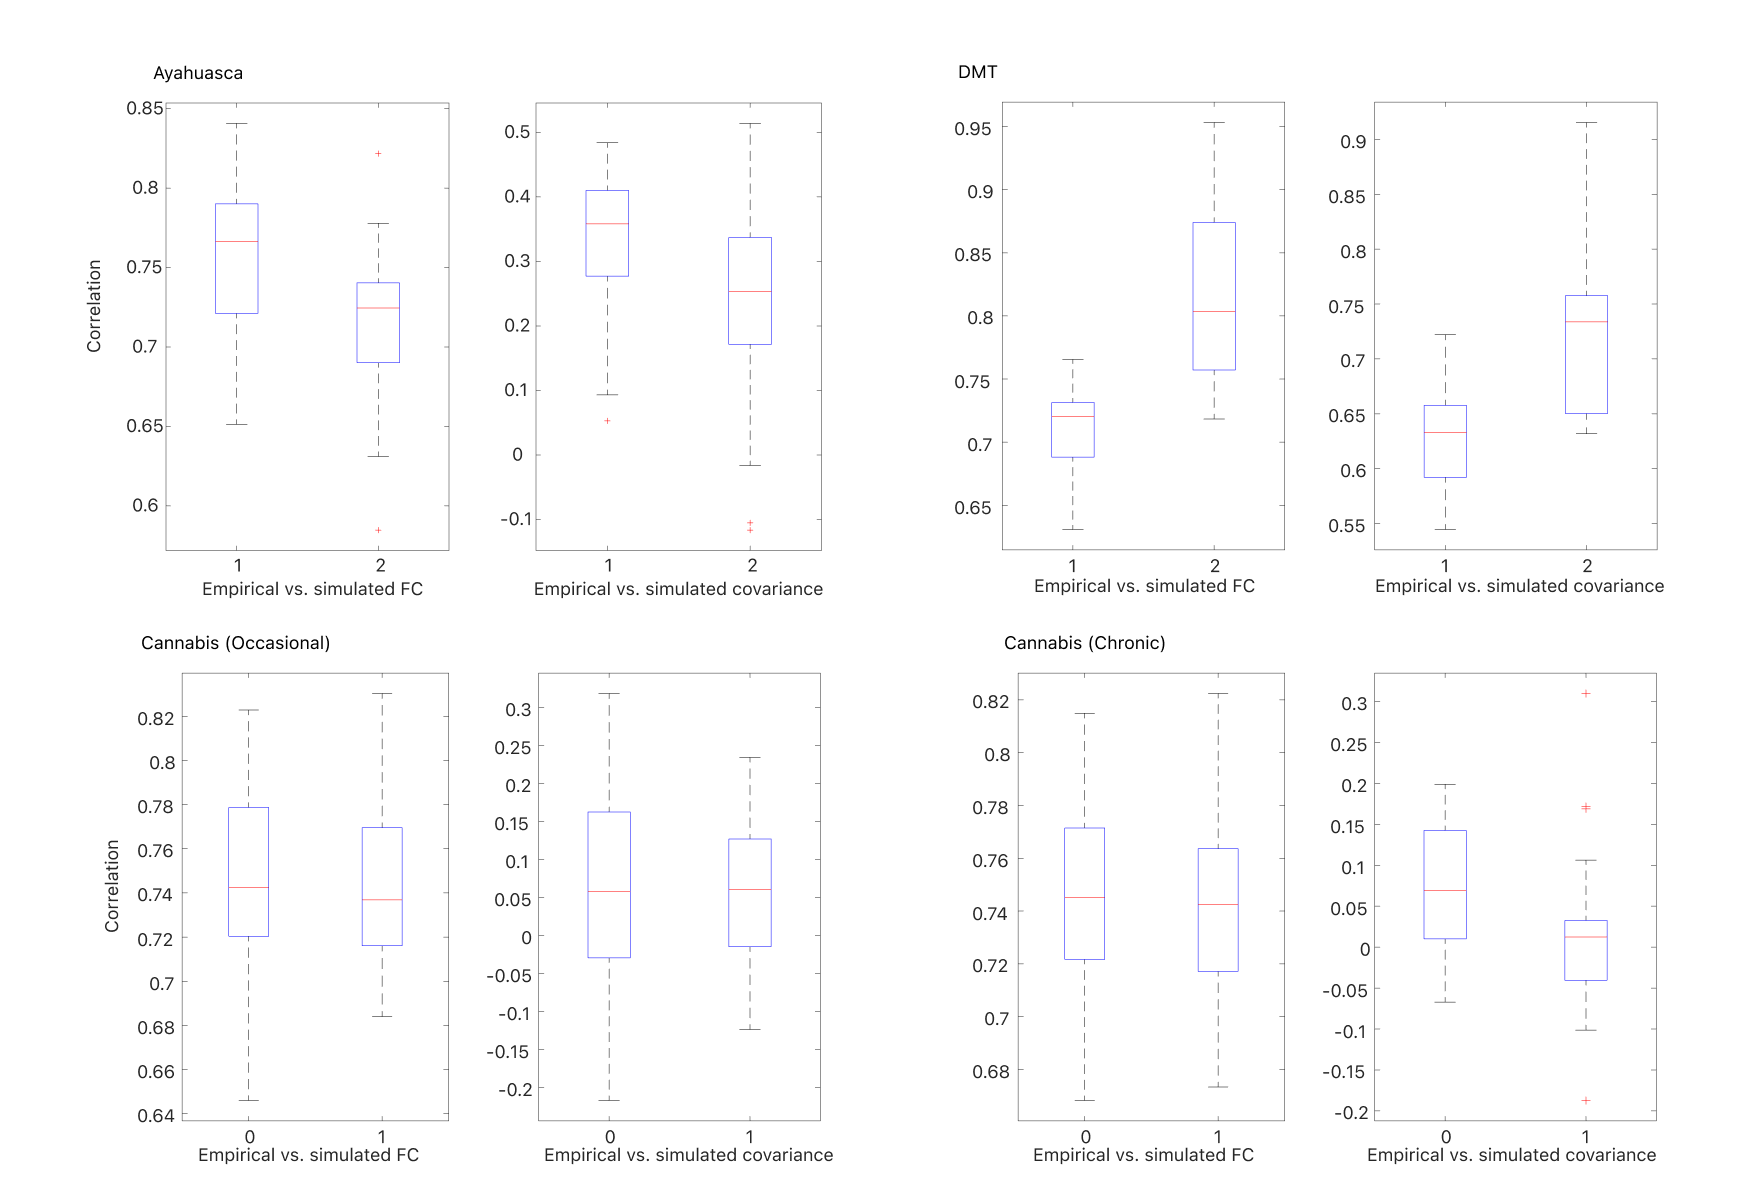
\includegraphics[width=\textwidth]{images/Appendix_ Fits.png}
    \caption[Whole-brain model fit.]{Correlations between empirical and simulated functional connectivity (left panel, each condition), and between empirical and simulated covariance of irreversibility matrices (right panel, each condition). "1" indicates baseline or placebo condition. "2" indicates drug condition.}
    \label{fig:fits}
\end{figure}

\begin{figure}[h!]
    \centering
    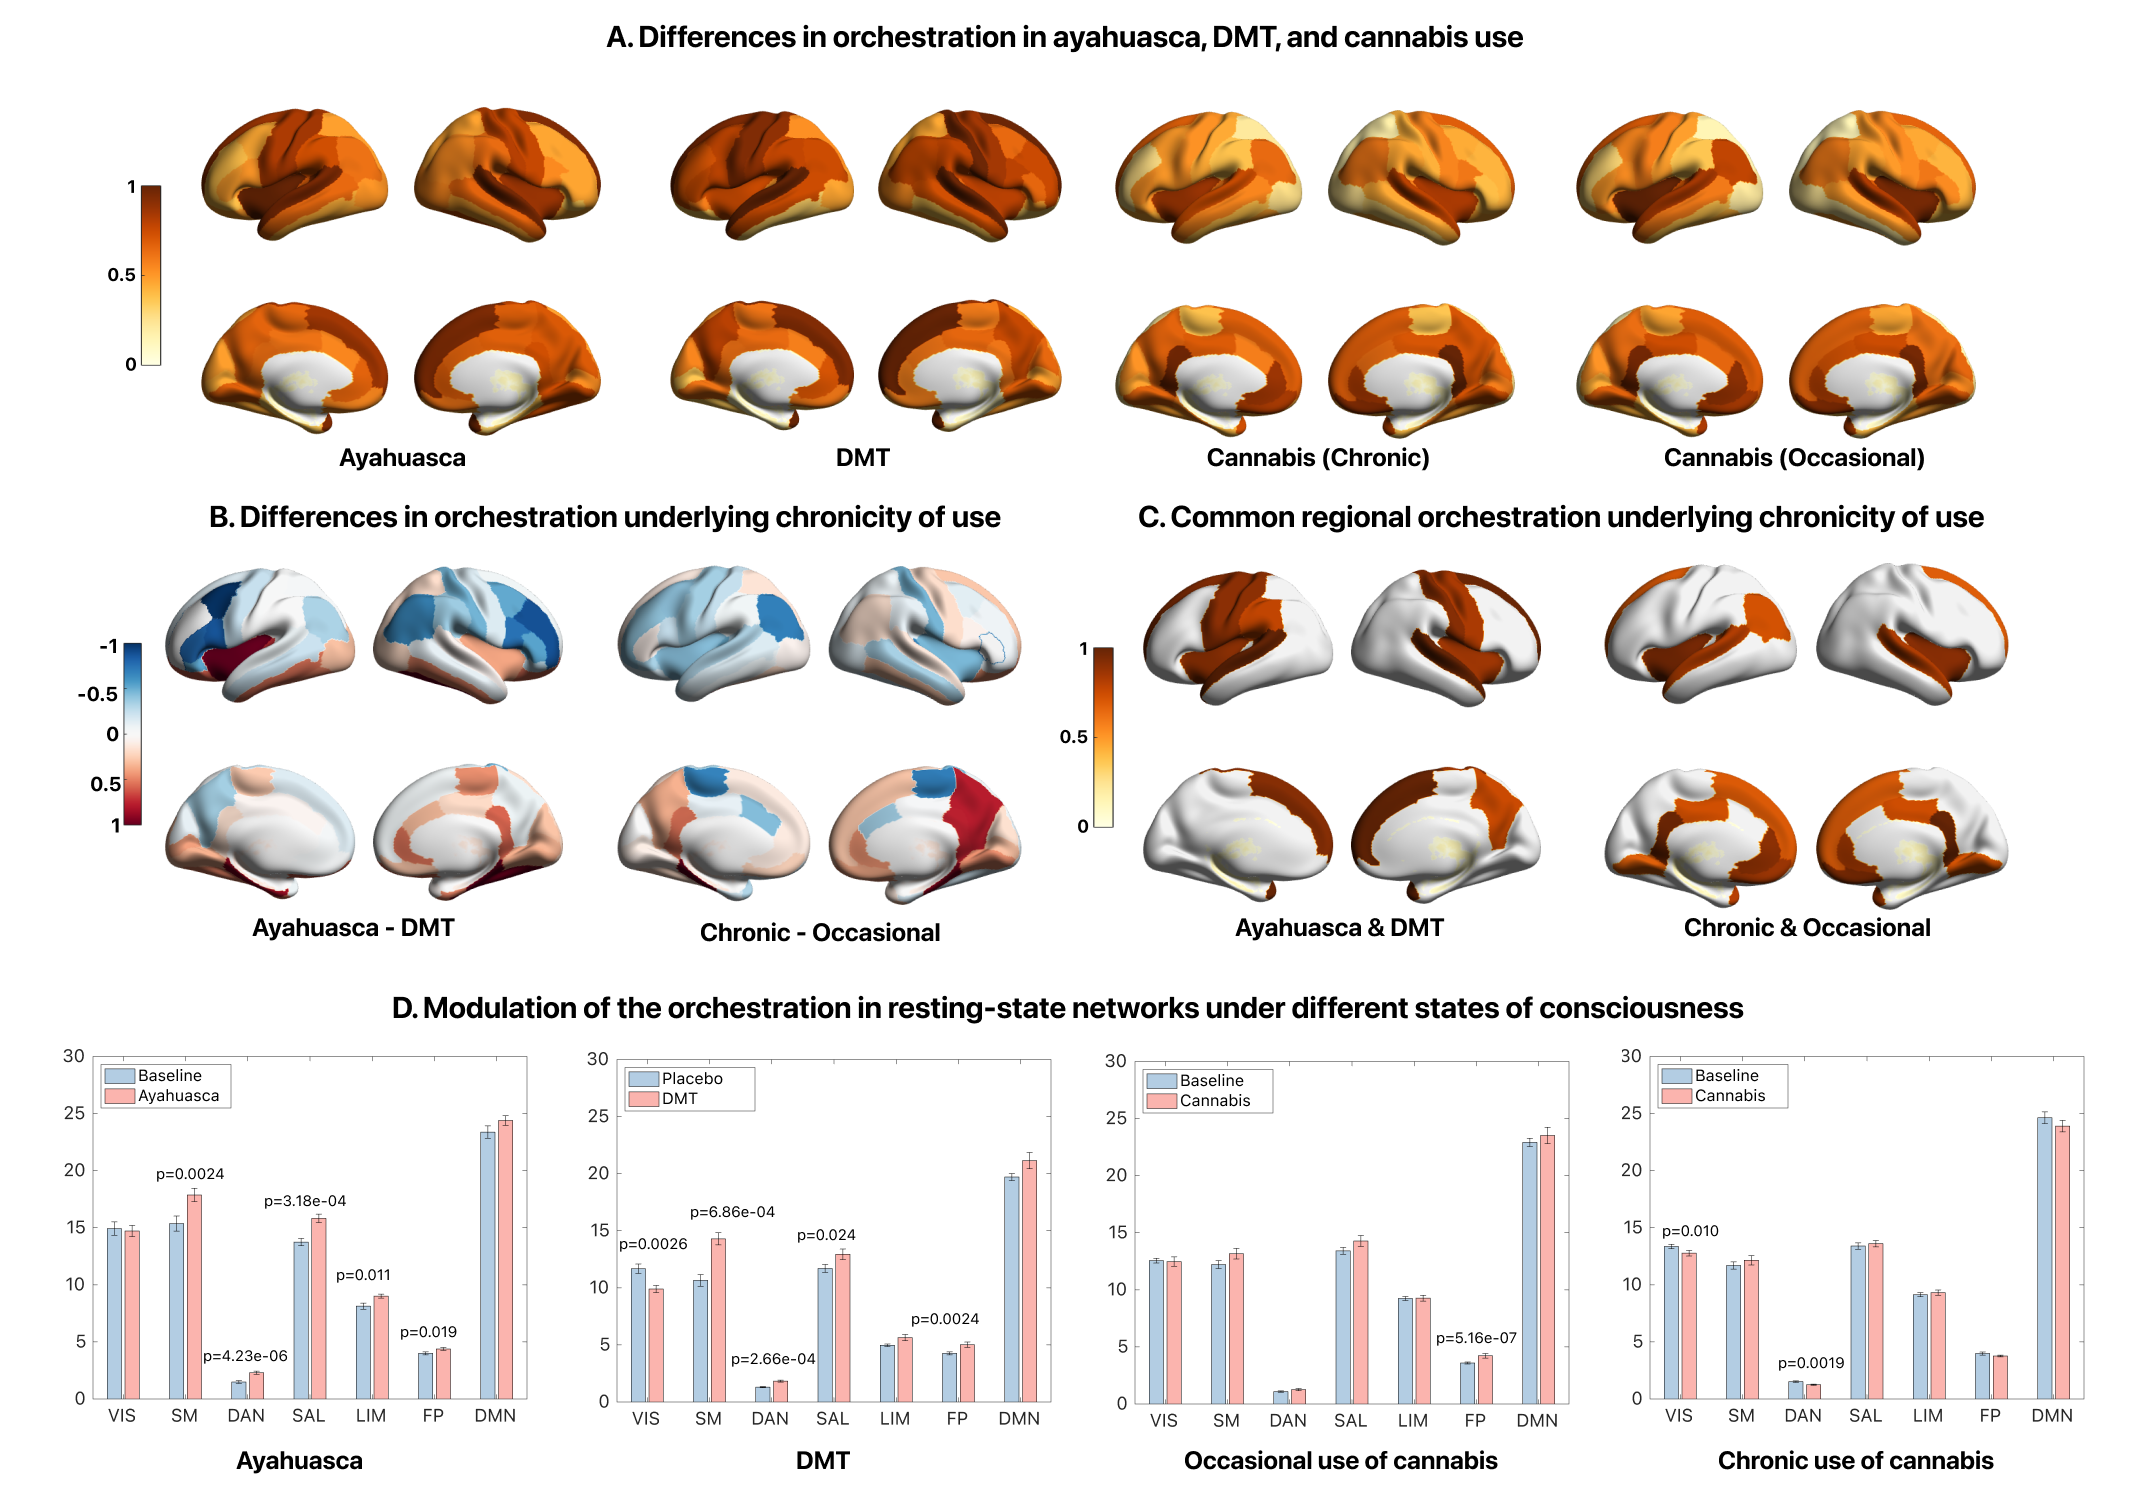
\includegraphics[width=\textwidth]{images/Appendix_GEC.png}
    \caption[Changes in directed connectivity in the psychedelic and cannabis states]{Differences in orchestration, a measure of total directed connectivity, under psychedelics and cannabis. (A) Measure of orchestration for each drug condition. Significant orchestrators for ayahuasca and DMT include bilateral pre- and post-central, insula, and superior frontal. For cannabis, bilateral insula, isthmus cingulate, and caudal anterior cingulate were found to be more connected than other regions in the brain. (B) Differences in orchestration between psychedelics, ayahuasca and DMT, and chronic and occasional use of cannabis. (C) Common orchestrators under psychedelics and cannabis. (D) Modulation of network-level orchestration under psychedelics and cannabis. Non-parametric permutation testing (5,000 iterations, threshold = 0.01) was utilized to evaluate changes in individual resting-state networks for each drug condition.}
    \label{fig:gecrender}
\end{figure}
\begin{figure}[h!]
    \centering
    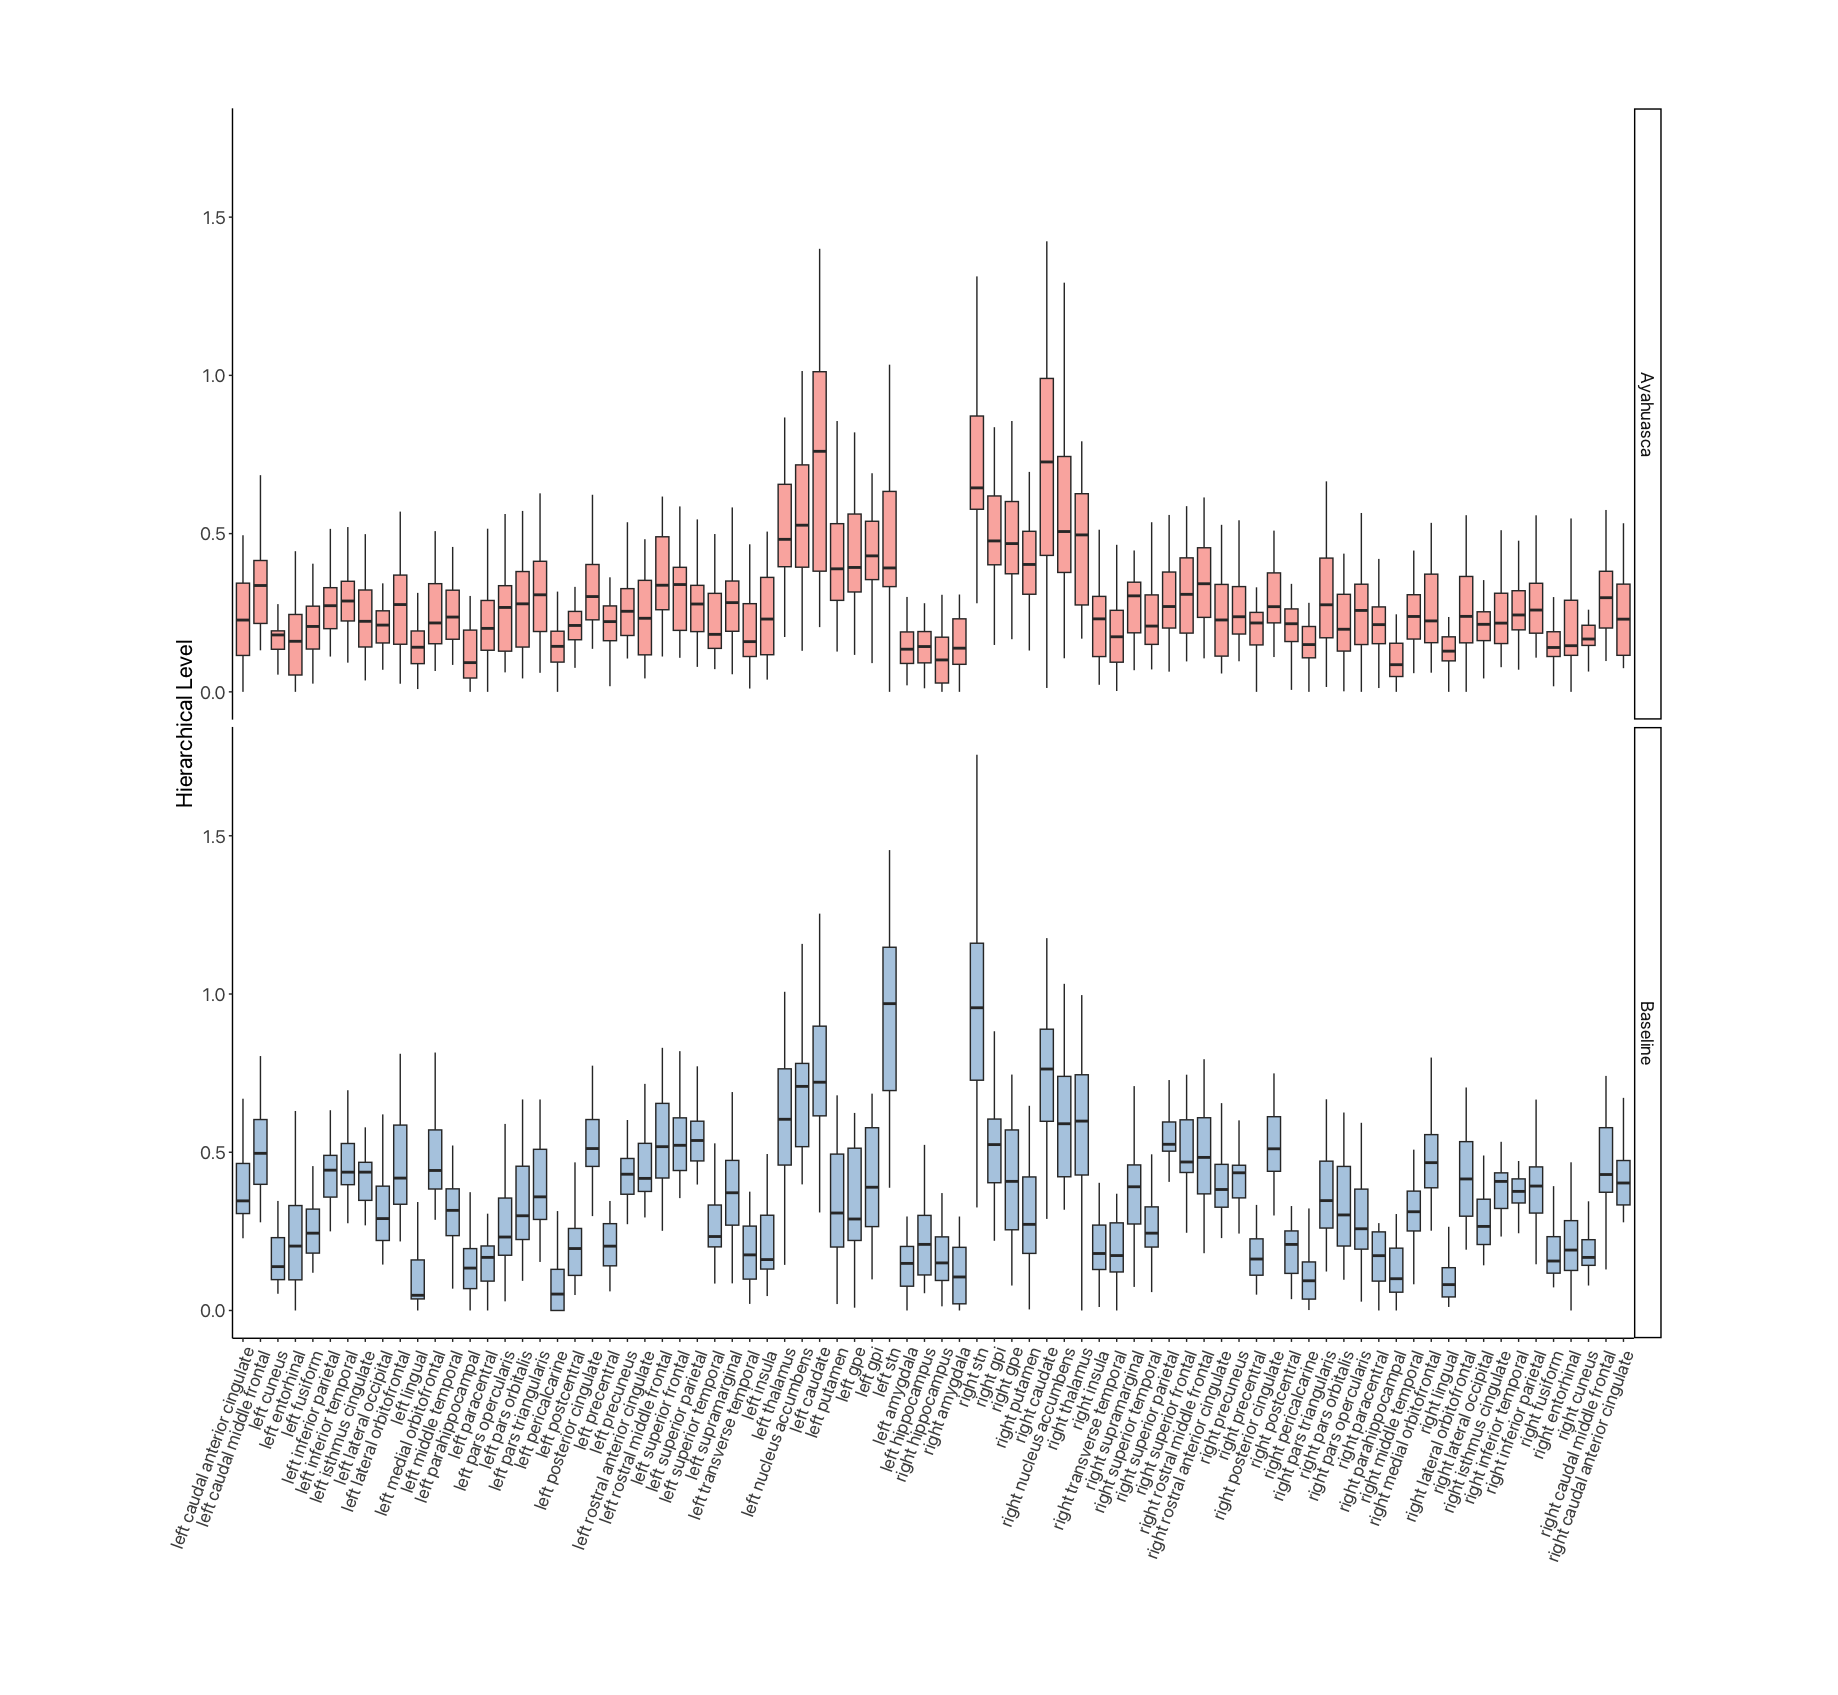
\includegraphics[width=\textwidth]{images/Appendix_ AYA HL.png}
    \caption[Regional hierarchical levels under baseline and ayahuasca.]{Hierarchical levels for each region in the DBS80 across baseline and ayahuasca conditions. Top panel, ayahuasca. Bottom panel, baseline.}
    \label{fig:ayahl}
\end{figure}

\begin{figure}[h!]
    \centering
    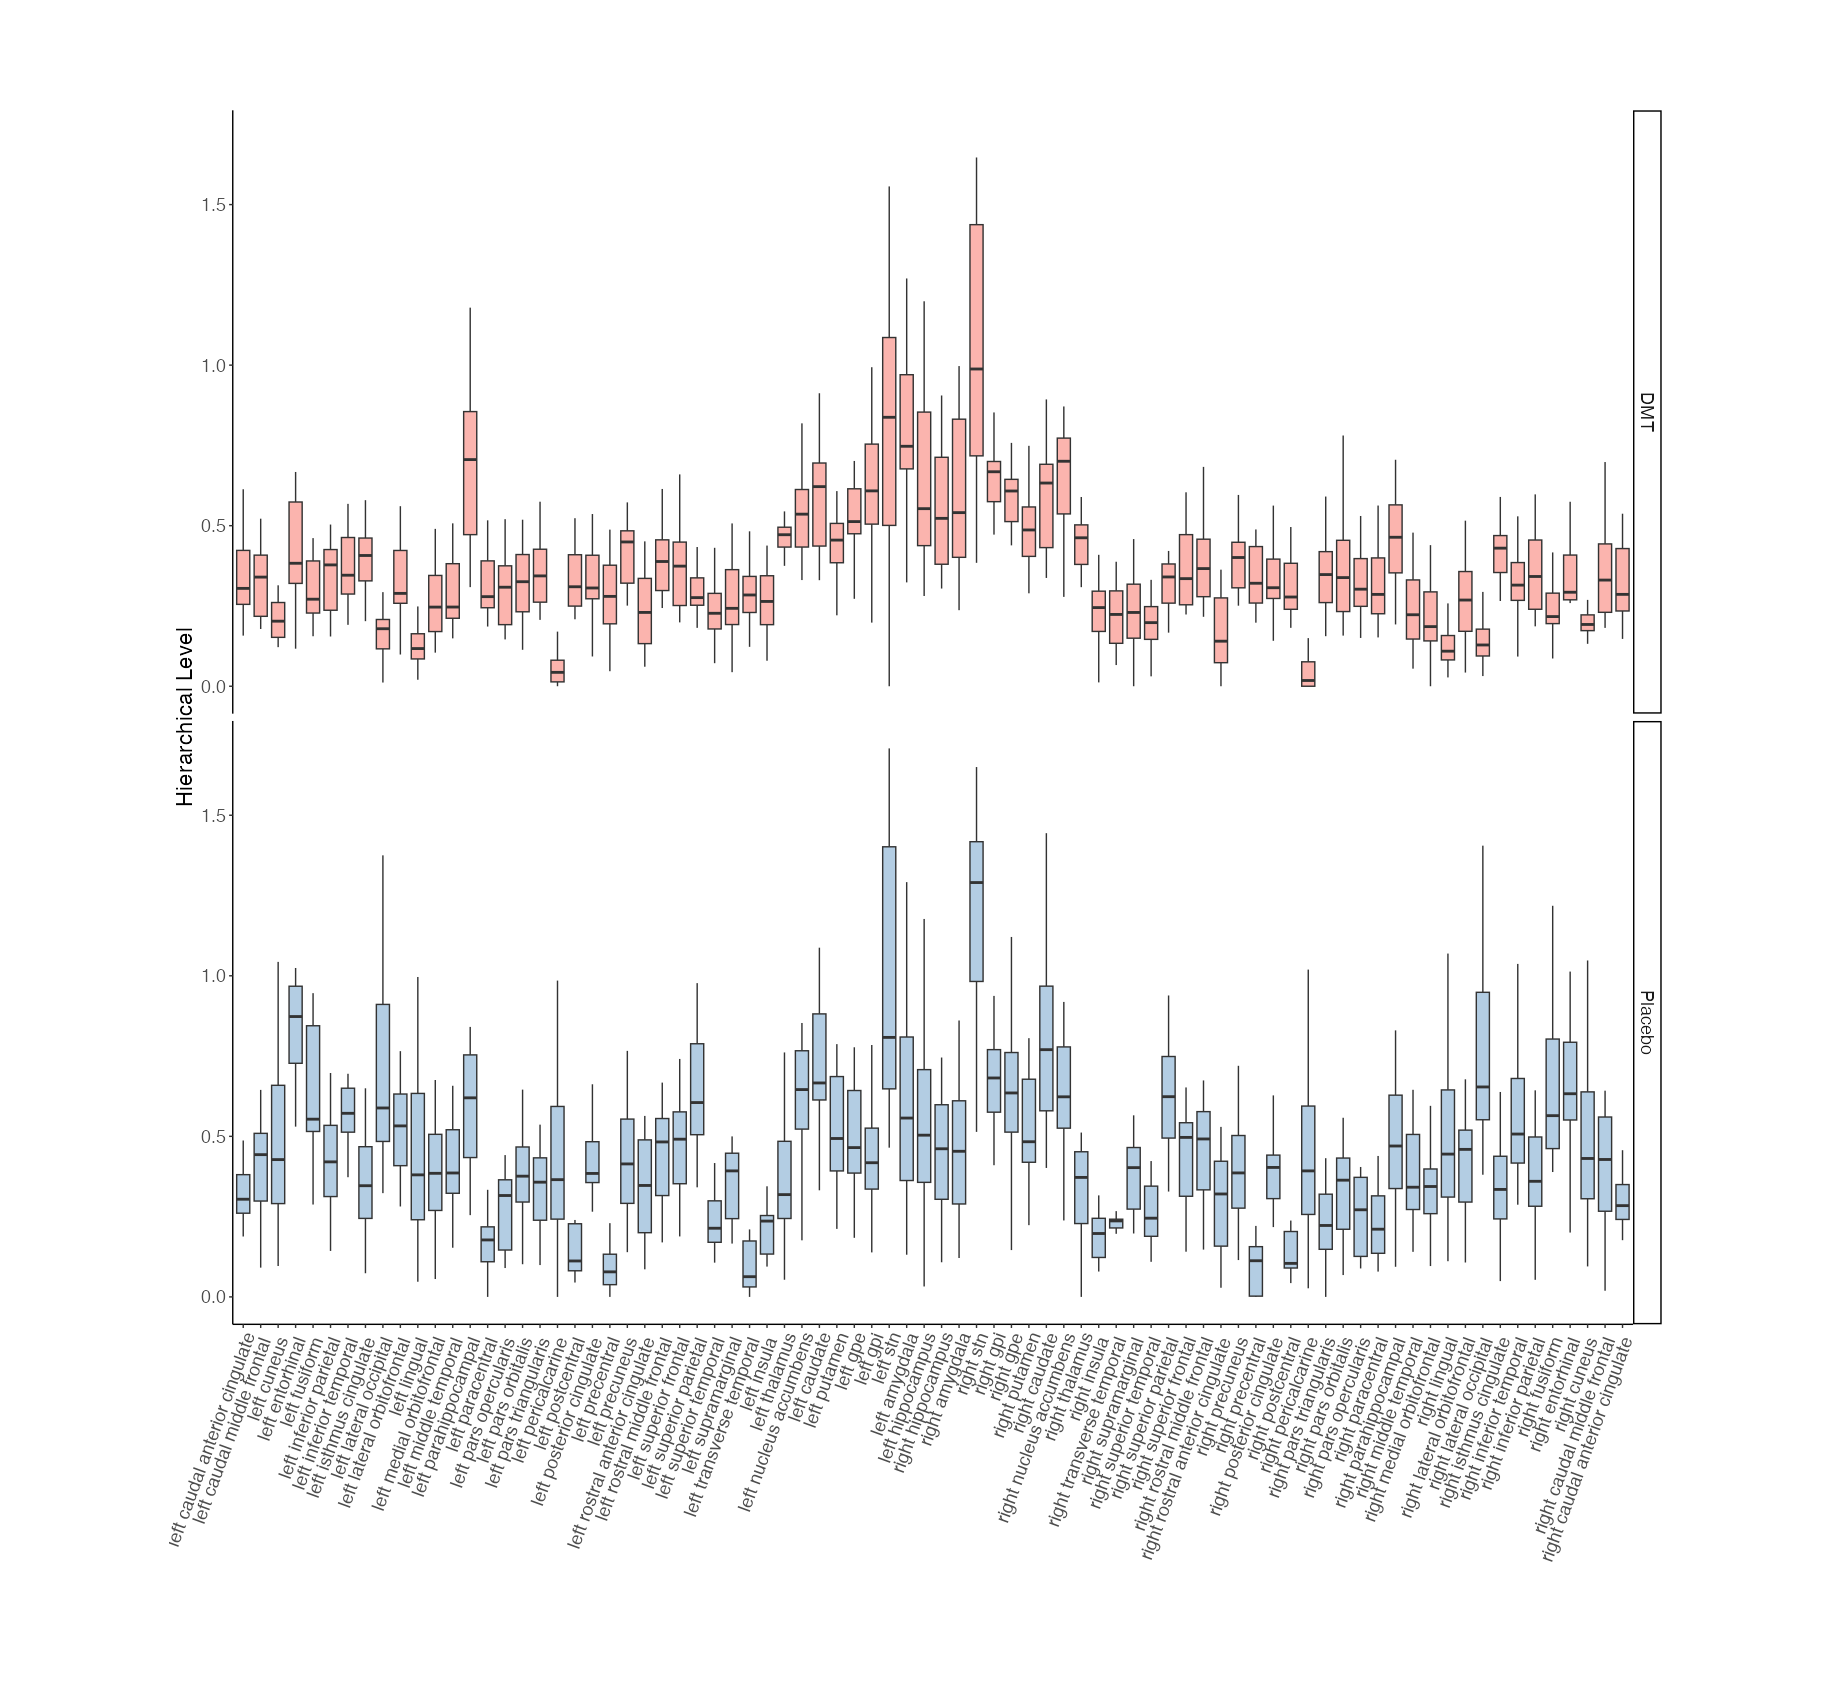
\includegraphics[width=\textwidth]{images/Appendix_ DMT HL.png}
    \caption[Hierarchical levels under placebo and DMT.]{Hierarchical levels for each region in the DBS80 across placebo and DMT conditions. Top panel, DMT. Bottom panel, placebo.}
    \label{fig:dmthl}
\end{figure}

\begin{figure}[h!]
    \centering
    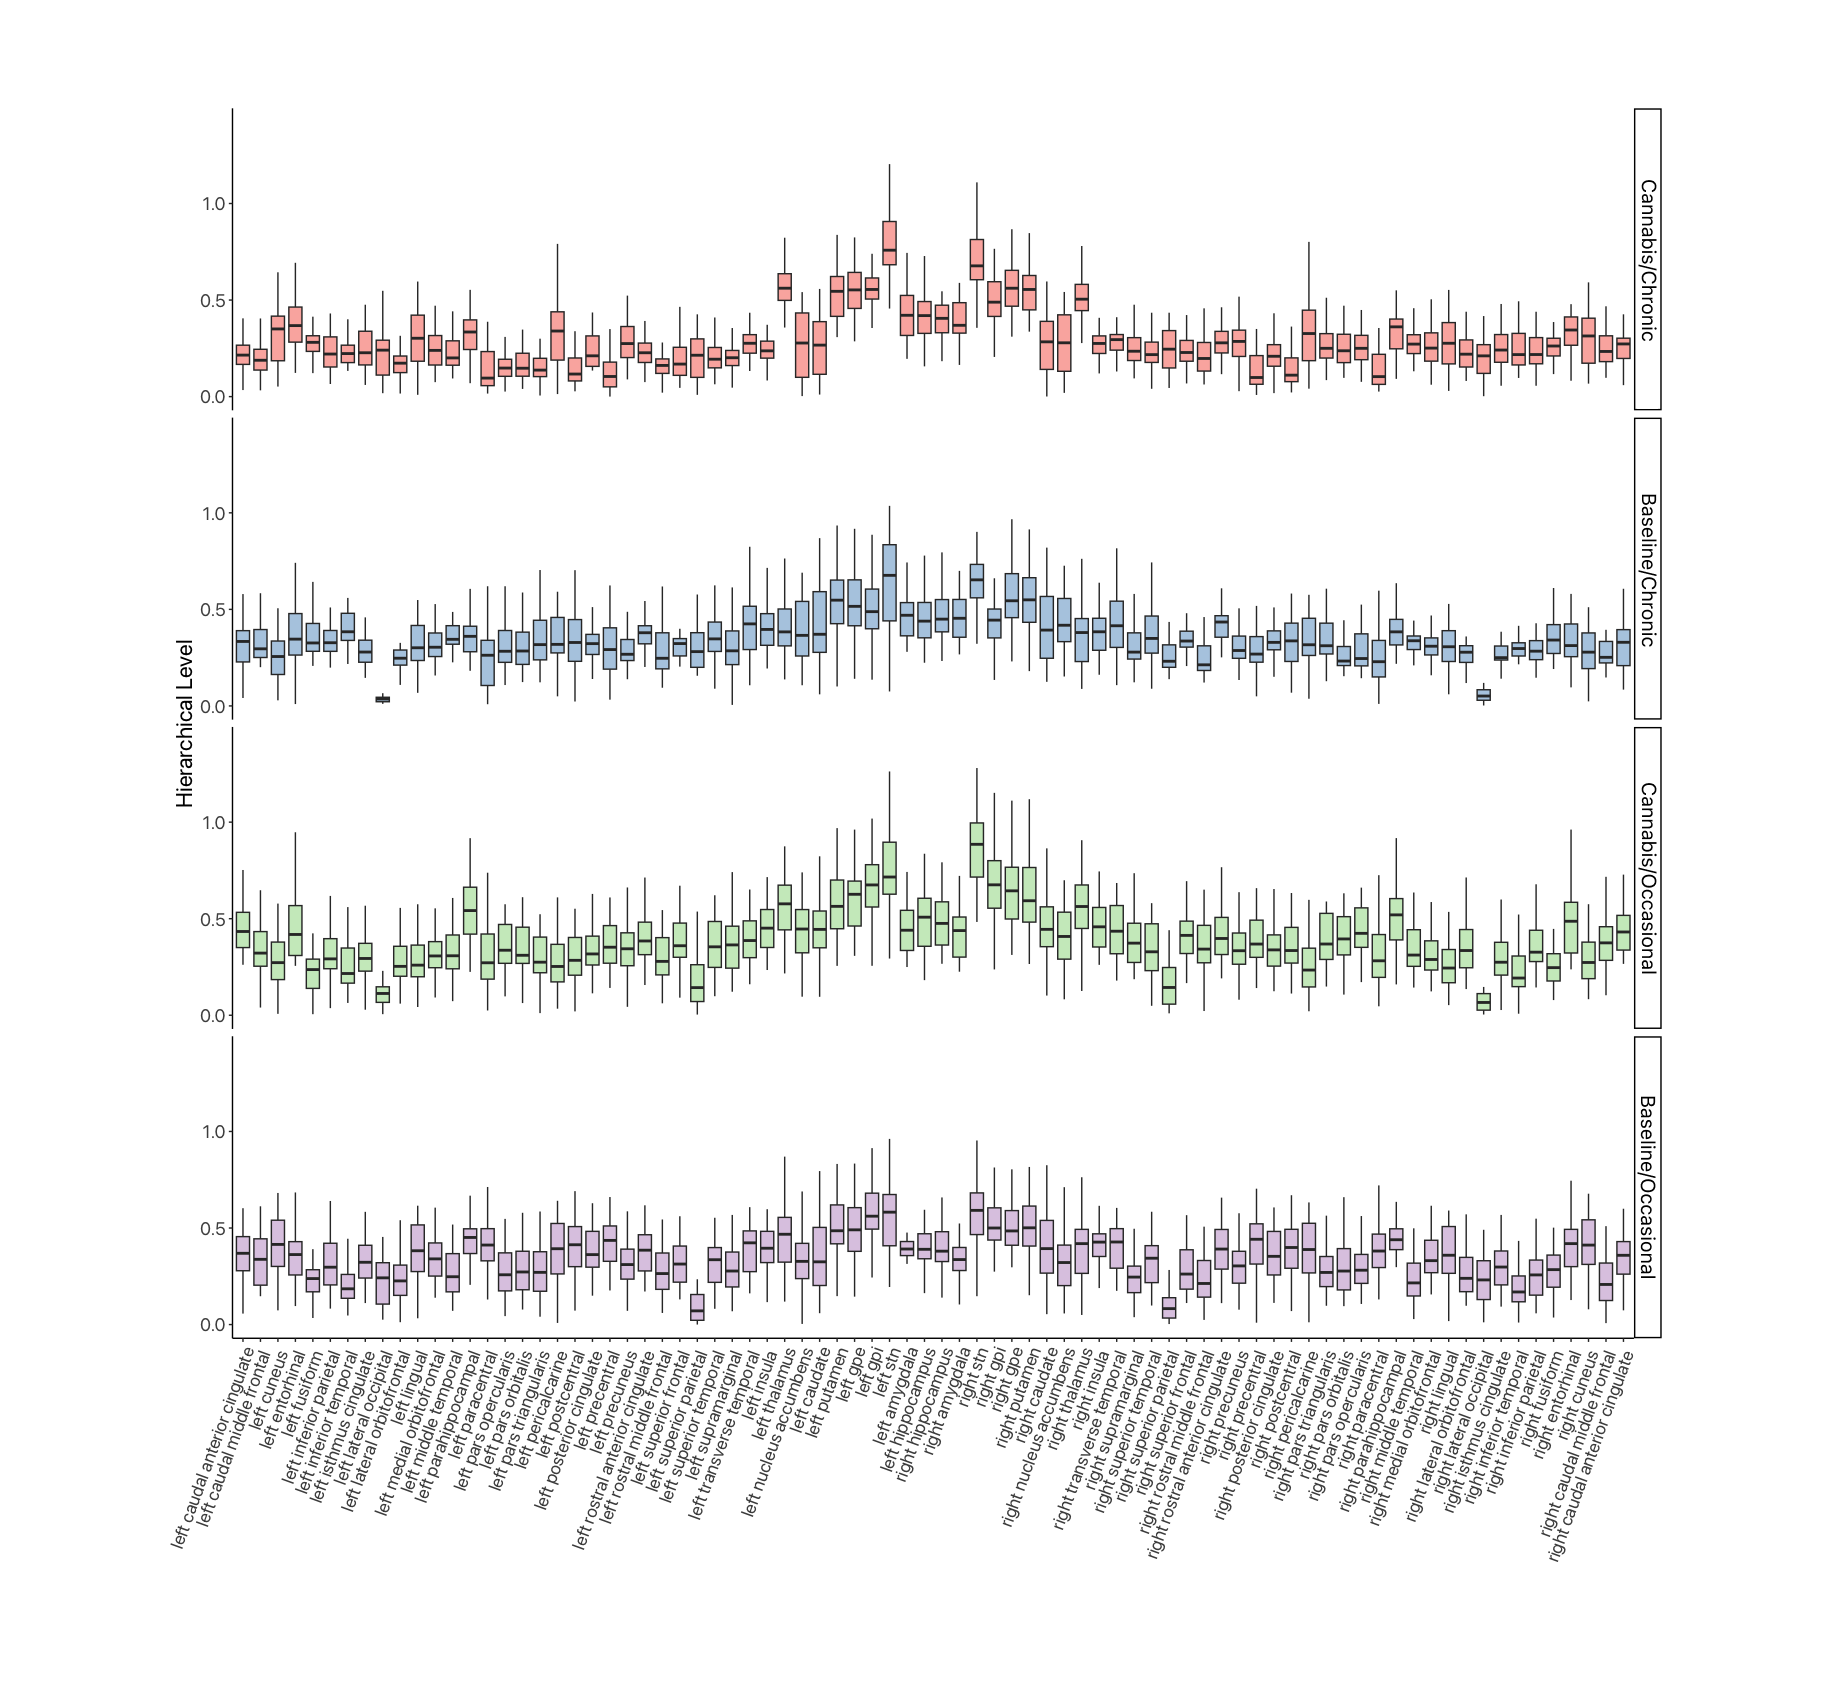
\includegraphics[width=\textwidth]{images/Appendix_ Cannab HL.png}
    \caption[Hierarchical levels under baseline and cannabis in chronic and occasional users.]{Hierarchical levels for each region in the DBS80 across baseline and cannabis (both chronic and occasional users). Top panel, cannabis in chronic users. Mid-top panel, baseline in chronic users. Mid-bottom panel, cannabis in occasional users. Bottom panel, baseline in occasional users.}
    \label{fig:cannabishl}
\end{figure}

\end{document}
